\documentclass[letterpaper,12pt]{article}
\usepackage{lipsum}  
\usepackage{graphicx}
\usepackage{subcaption}
\usepackage[english]{babel}
\usepackage{fancyhdr}
\usepackage{pdfpages}
\usepackage{hyperref}
\usepackage{afterpage}
\usepackage{appendix}
\usepackage[utf8]{inputenc} 
\usepackage{listings}
\usepackage{color}
 
\definecolor{codegreen}{rgb}{0,0.6,0}
\definecolor{codegray}{rgb}{0.5,0.5,0.5}
\definecolor{codepurple}{rgb}{0.58,0,0.82}
\definecolor{backcolour}{rgb}{0.95,0.95,0.92}

\graphicspath {{figures/}}

\setlength{\headheight}{15pt}

\pagestyle{fancy}
\fancyhf{}
\lhead{\textbf{Version:} 1.0  \textbf{Revision:} \today}
%\lhead{\textbf{Version:} 1.0  \textbf{Revision:} 01/23/18}
\rhead{\thepage}
\lfoot{Cole Kampa}
\rfoot{\textit{Mu2e: University of Minnesota}}

\renewcommand{\footrulewidth}{1pt}

\lstdefinestyle{mystyle}{
    backgroundcolor=\color{backcolour},   
    commentstyle=\color{codegreen},
    keywordstyle=\color{magenta},
    numberstyle=\tiny\color{codegray},
    stringstyle=\color{codepurple},
    basicstyle=\footnotesize,
    breakatwhitespace=false,         
    breaklines=true,                 
    captionpos=b,                    
    keepspaces=true,                 
    numbers=left,                    
    numbersep=5pt,                  
    showspaces=false,                
    showstringspaces=false,
    showtabs=false,                  
    tabsize=2
}
 
\lstset{style=mystyle}

\begin{document}
\begin{titlepage}
	\centering
	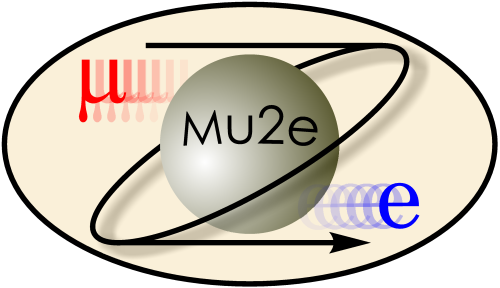
\includegraphics[width=0.5\textwidth]{mu2e_logo_oval.png}\par\vspace{2cm}
	{\scshape\LARGE Threader Documentation\par}
	\vspace{3cm}
	{\Large Cole Kampa\par}
	\vspace{3cm}
	{\large University of Minnesota\par}
 	\vspace{.5cm}
	{\large \today \par}
%	{\large January 23, 2018\par}
	% Bottom of the page
	\vfill
	{kampa041@umn.edu\par}
\end{titlepage}

\setcounter{page}{2}

\tableofcontents
\clearpage

\section{Goal}
We aim to design a robust and scalable device that can run thread through straws epoxied in a panel. Sense wire will be hot glued onto thread and pulled through each straw. We strive to do this in a safe, efficient, and reproducible manner.


\section{Device Overview}
There are two main components to the threader unit. The 'gun', which the user controls, is a pistol grip blow gun connected to nitrogen and various electronic components. A DC motor is housed on the gun, and spins a spool of thread. A small hole in the tip of the gun allows the thread to pass through. The nitrogen blows the thread along, while the motor allows more thread to be released. A potentiometer with a custom attachment controls the speed of the thread. A simple pushbutton allows the user to toggle the motor direction. \par
The gun has a plastic tube and Ethernet	 cable leading out of the base which go into the nitrogen cylinder and 'electronics box', respectively. The electronics box currently consists of a Arduino Micro which controls a Pololu Qik 2s9v1 dual serial motor controller. The potentiometer and pushbutton are wired into the Arduino, while the motor is wired into the output of the Pololu. The electronics are powered by a rechargeable 12V battery. Everything is kept on a cart, but the cart is currently tied to the large nitrogen cylinder in the lab. See the future updates section for more information on plans to mobilize the cart. The first version of the cart is shown in figure~\ref{fig:full_cart}.
\begin{figure} [h!]
		\centering
		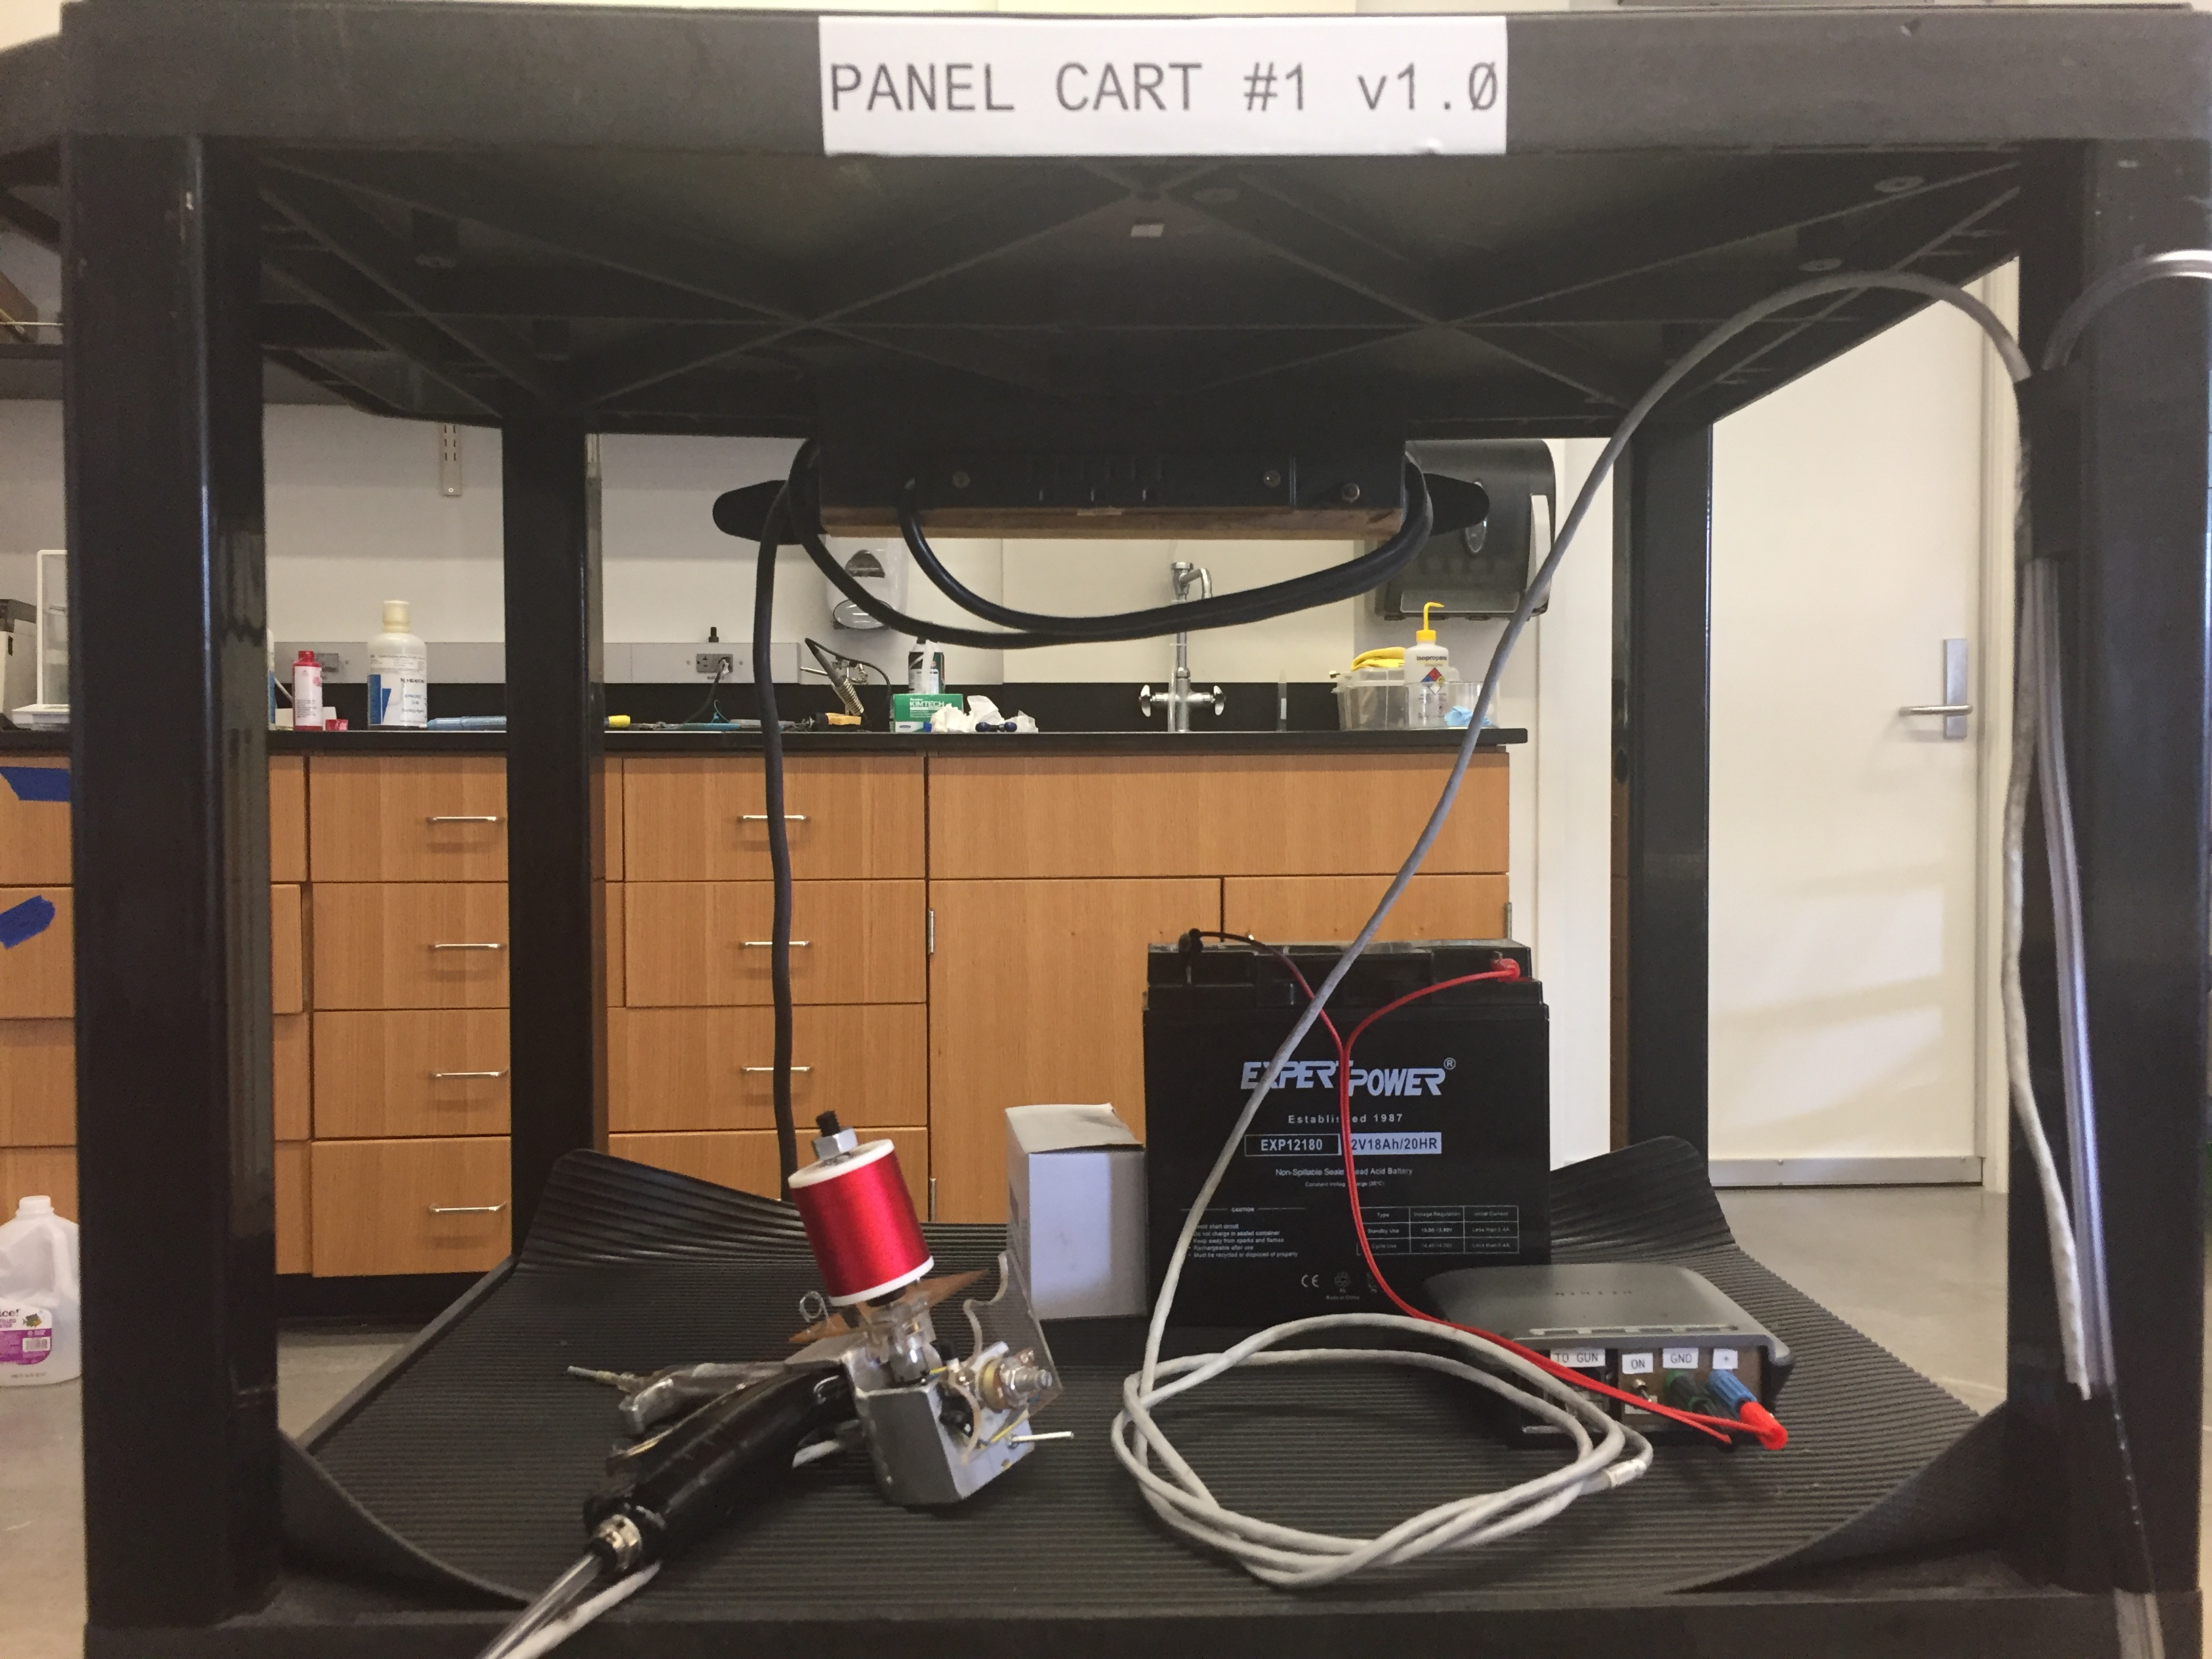
\includegraphics[width=1\textwidth]{cart_close.JPG}
		\caption{Full cart setup.}
		\label{fig:full_cart}
\end{figure}


\section{Basic Usage}
Note: Instructions for the standard tip. Other tip designs are still being developed.
\subsection{Setup}
Before operating the threader, the gas and electronics box must be turned on. The nitrogen cylinder and pressure gauges are shown in figure~\ref{fig:gas}. First, turn the valve on the nitrogen cylinder at least 1/2 turn counterclockwise. Then, turn the valve immediately to the right of the 'T' created by the hose from the tank to the regulators 1/2 turn counterclockwise. The bottom left gauge and top gauge should read non-zero values at this point. The bottom gauge should give a good indication of the amount of gas left in the tank, while the top gauge indicates the pressure to the gun. To adjust this pressure, turn the topmost valve (immediately underneath the top gauge) clockwise to increase pressure or counterclockwise to decrease pressure. \par
\afterpage{
\begin{figure} [h!]
		\centering
		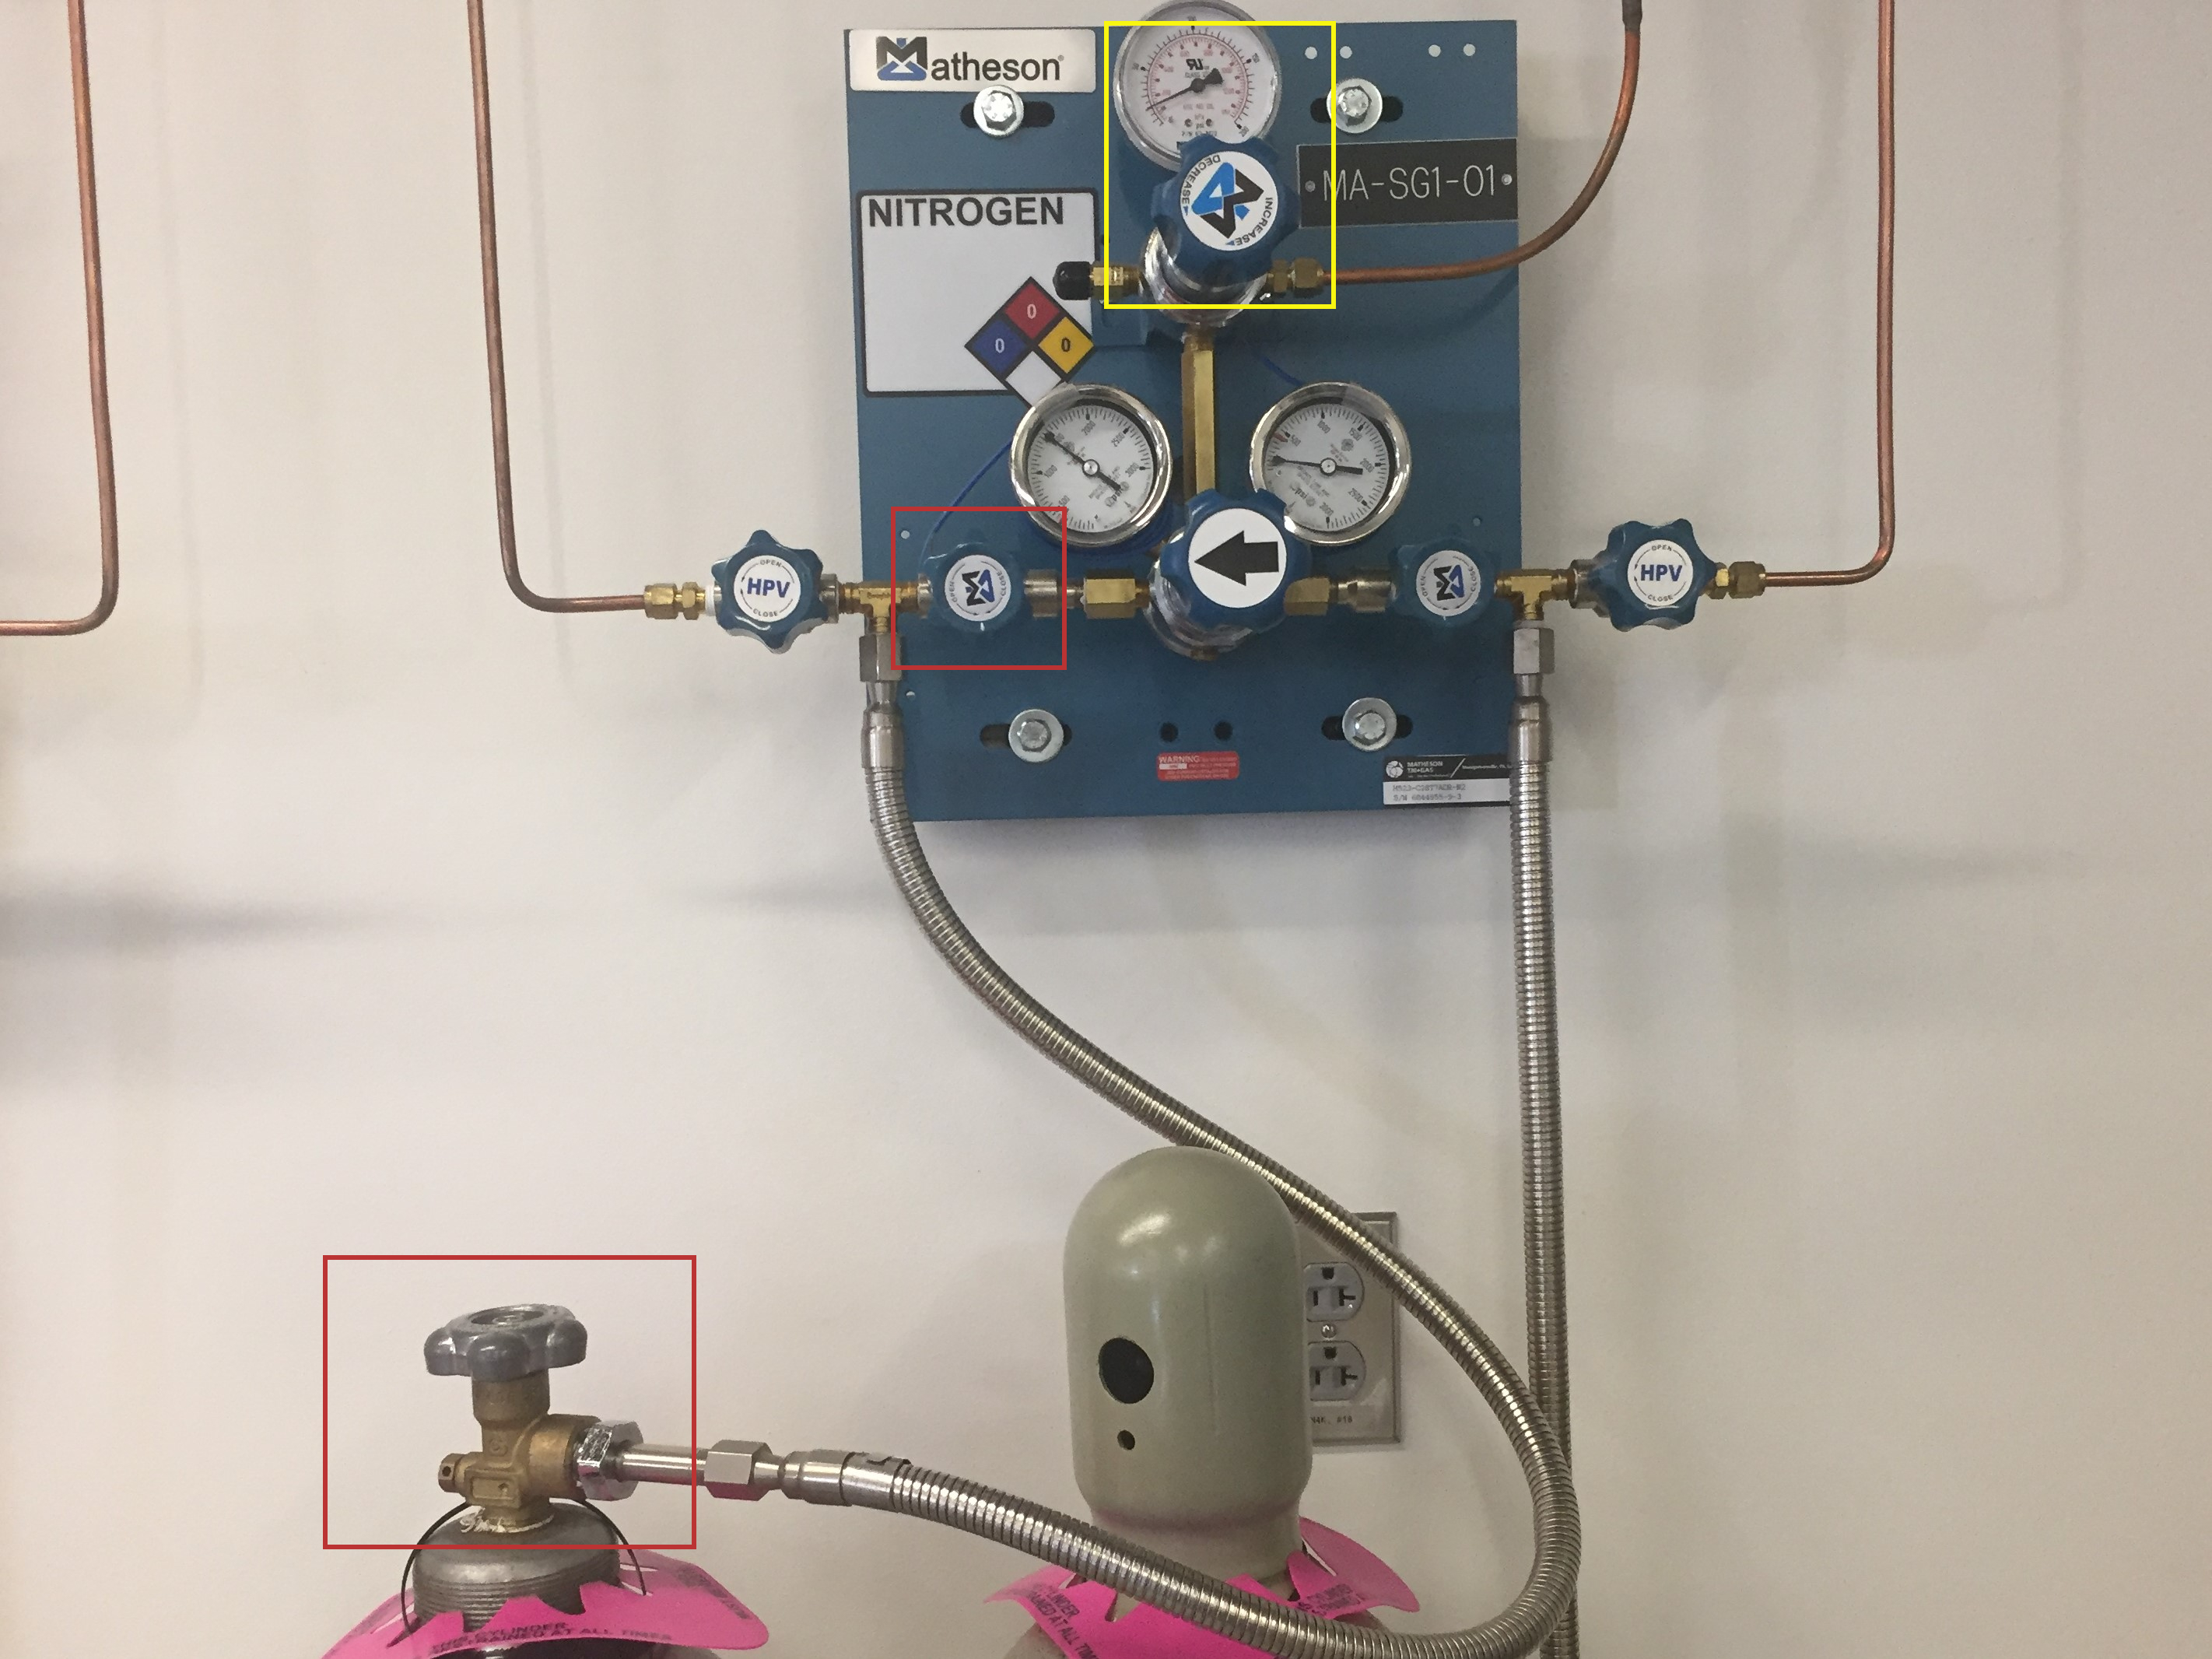
\includegraphics[width=0.75\textwidth]{gas_setup_label.JPG}
		\caption{Nitrogen tank and gauges in northwest corner of PAN 450. \underline{Red:} valves used in normal operation; \underline{Yellow:} valve and gauge used for controlling gun pressure.}
		\label{fig:gas}
\end{figure}
\begin{figure} [h!]
		\centering
		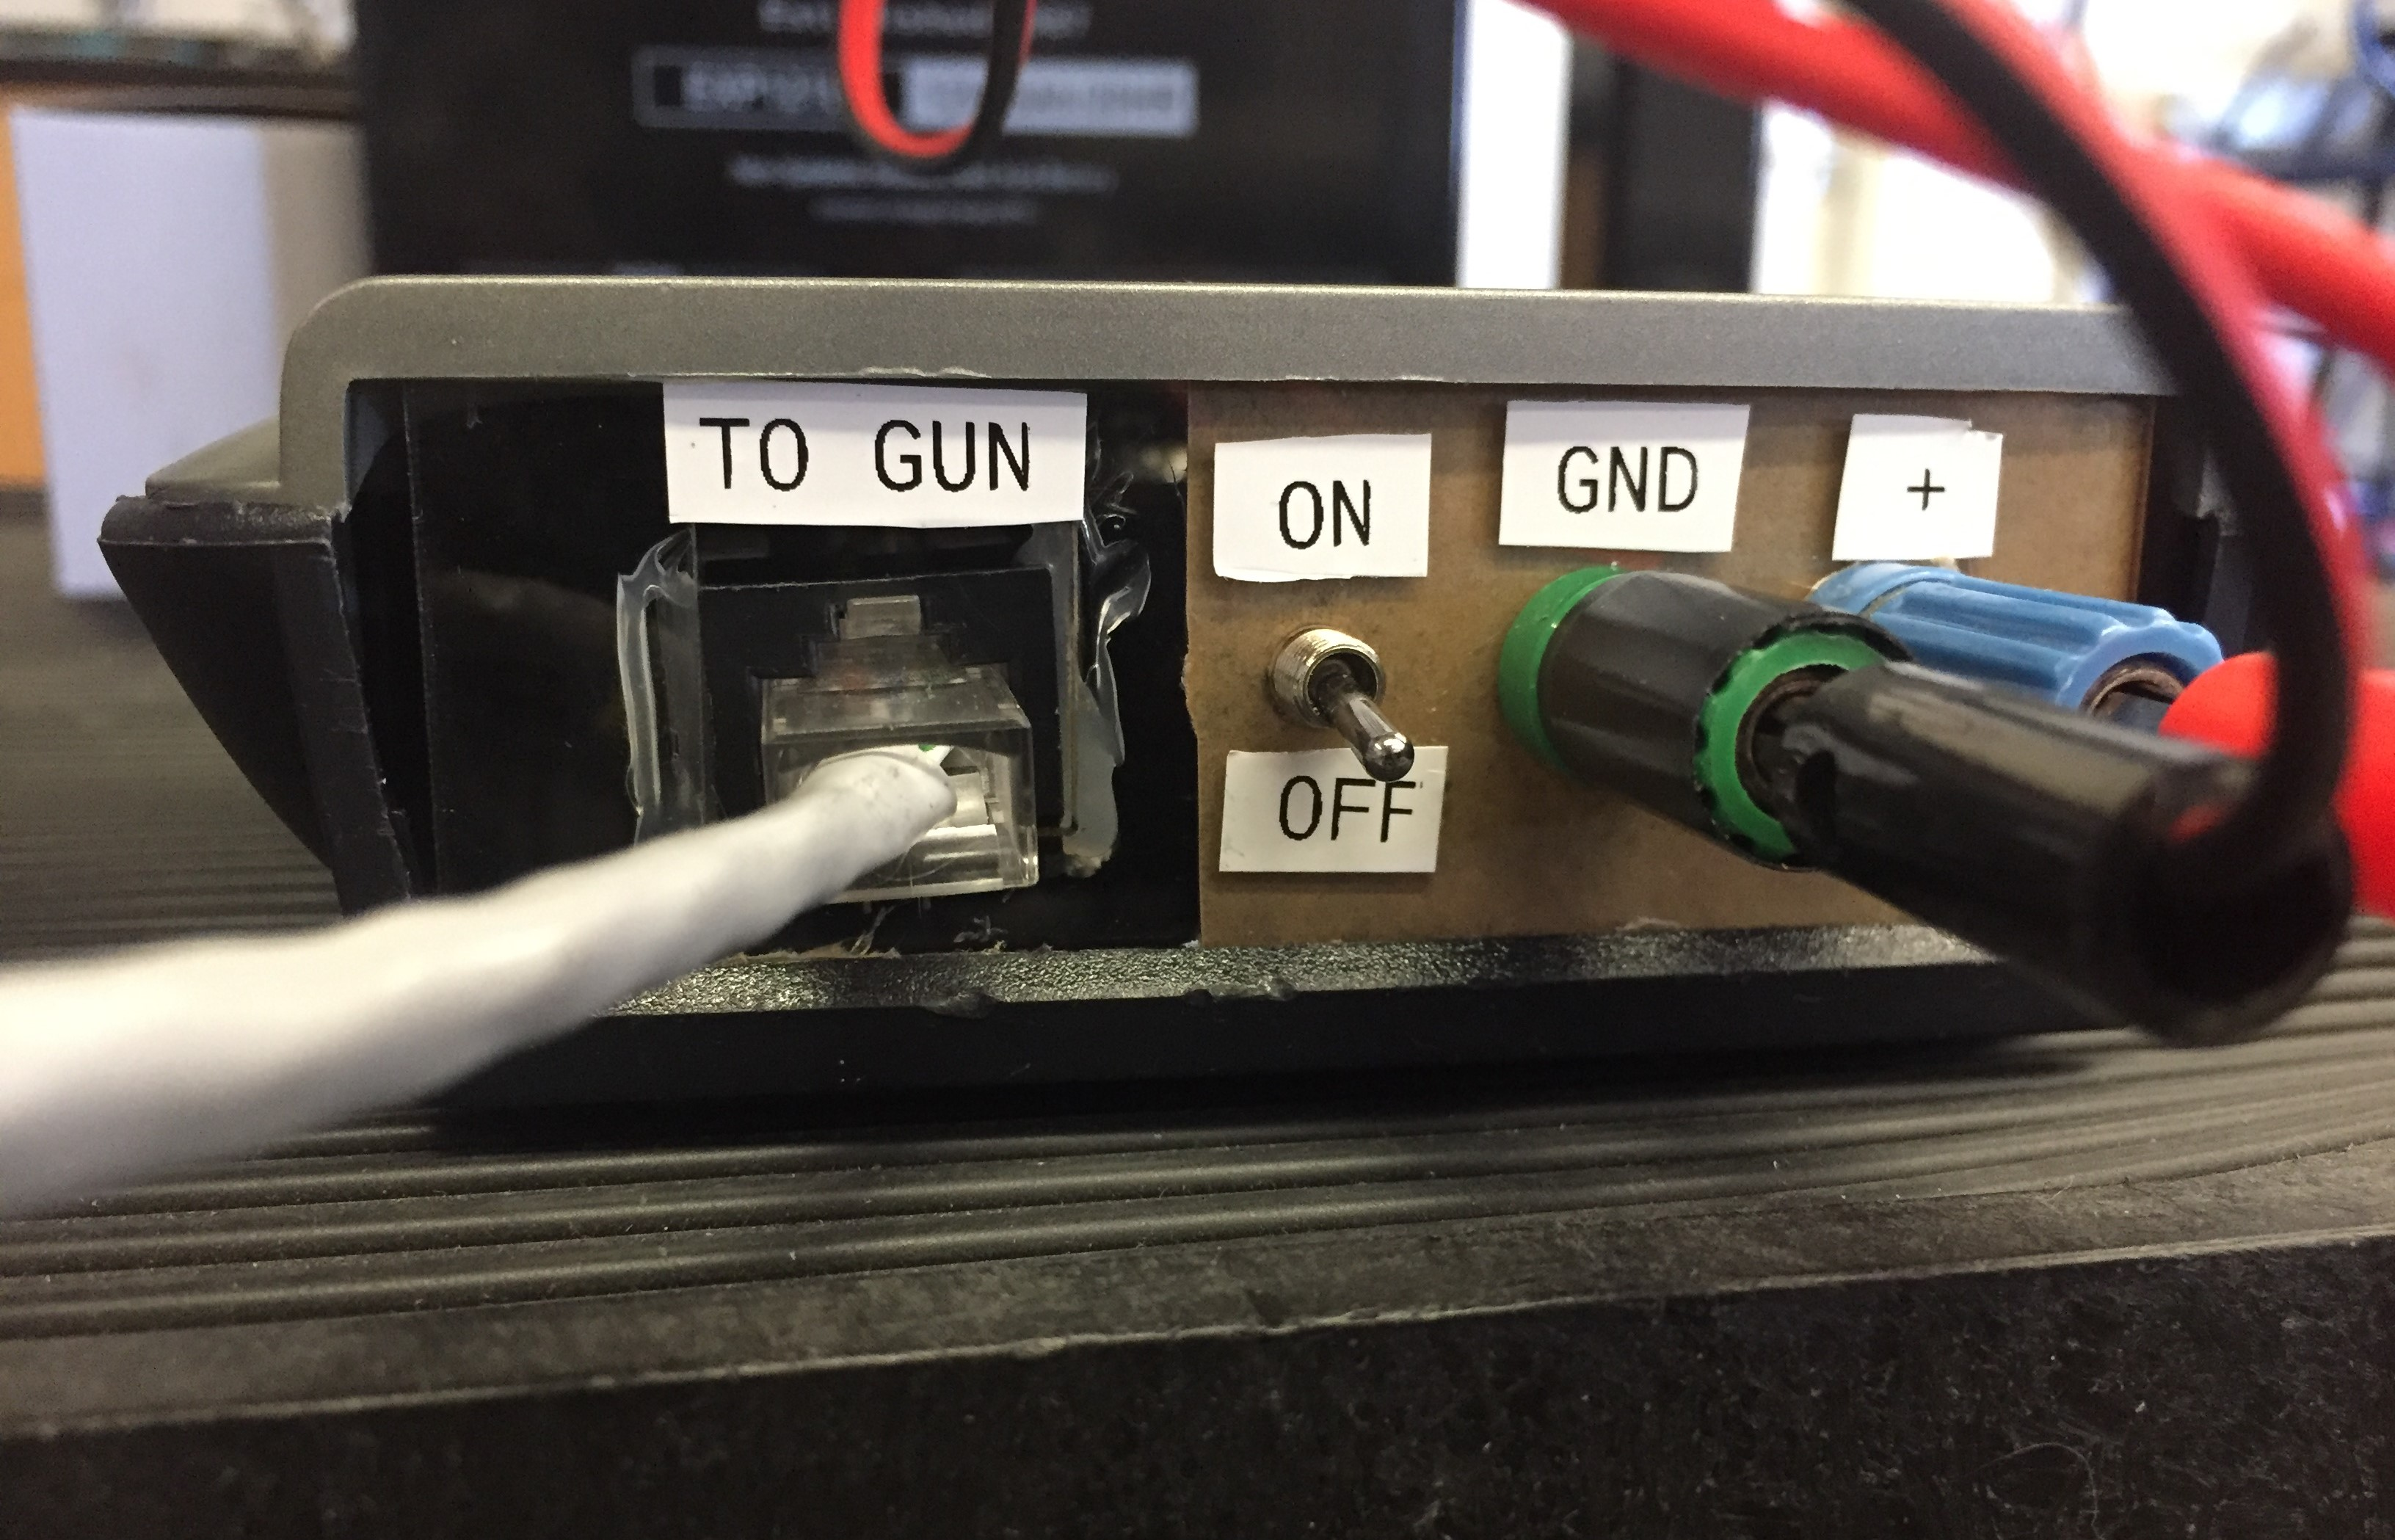
\includegraphics[width=0.75\textwidth]{front_plate.JPG}
		\caption{Front plate of the electronics box with everything properly plugged in.}
		\label{fig:box_front}
\end{figure}
\clearpage
}
To power the electronics, first verify that the gun and battery are plugged into the box (figure~\ref{fig:box_front}). Whenever adjusting the power cables, be careful to not short circuit the battery. Accordingly, it is safest to first plug the banana plugs into the box, then the alligator clips to the battery. If you must unplug the unit, unplug the alligator clips on the battery first. Now that the cabling is properly in place, turn on the device by flipping the silver toggle switch on the front plate of the electronics box to the 'on' position. The Plexiglass speed control wheel on the back of the gun is adjusted by the user each time a straw is threaded. The speed control wheel not only controls the speed, but also whether the motor is on or off (see figure~\ref{fig:speed}). To check that the electronics are functional, turn the speed control wheel on the back of the gun. This should cause the spool to spin. While the motor is on, try pressing the motor reversal button. If both of these functions work, the gun electronics are working. Finish this preparation step by ensuring the motor is spinning forward (thread is released). \par
\begin{figure}[h!]
\centering
\begin{subfigure}{.5\textwidth}
  \centering
  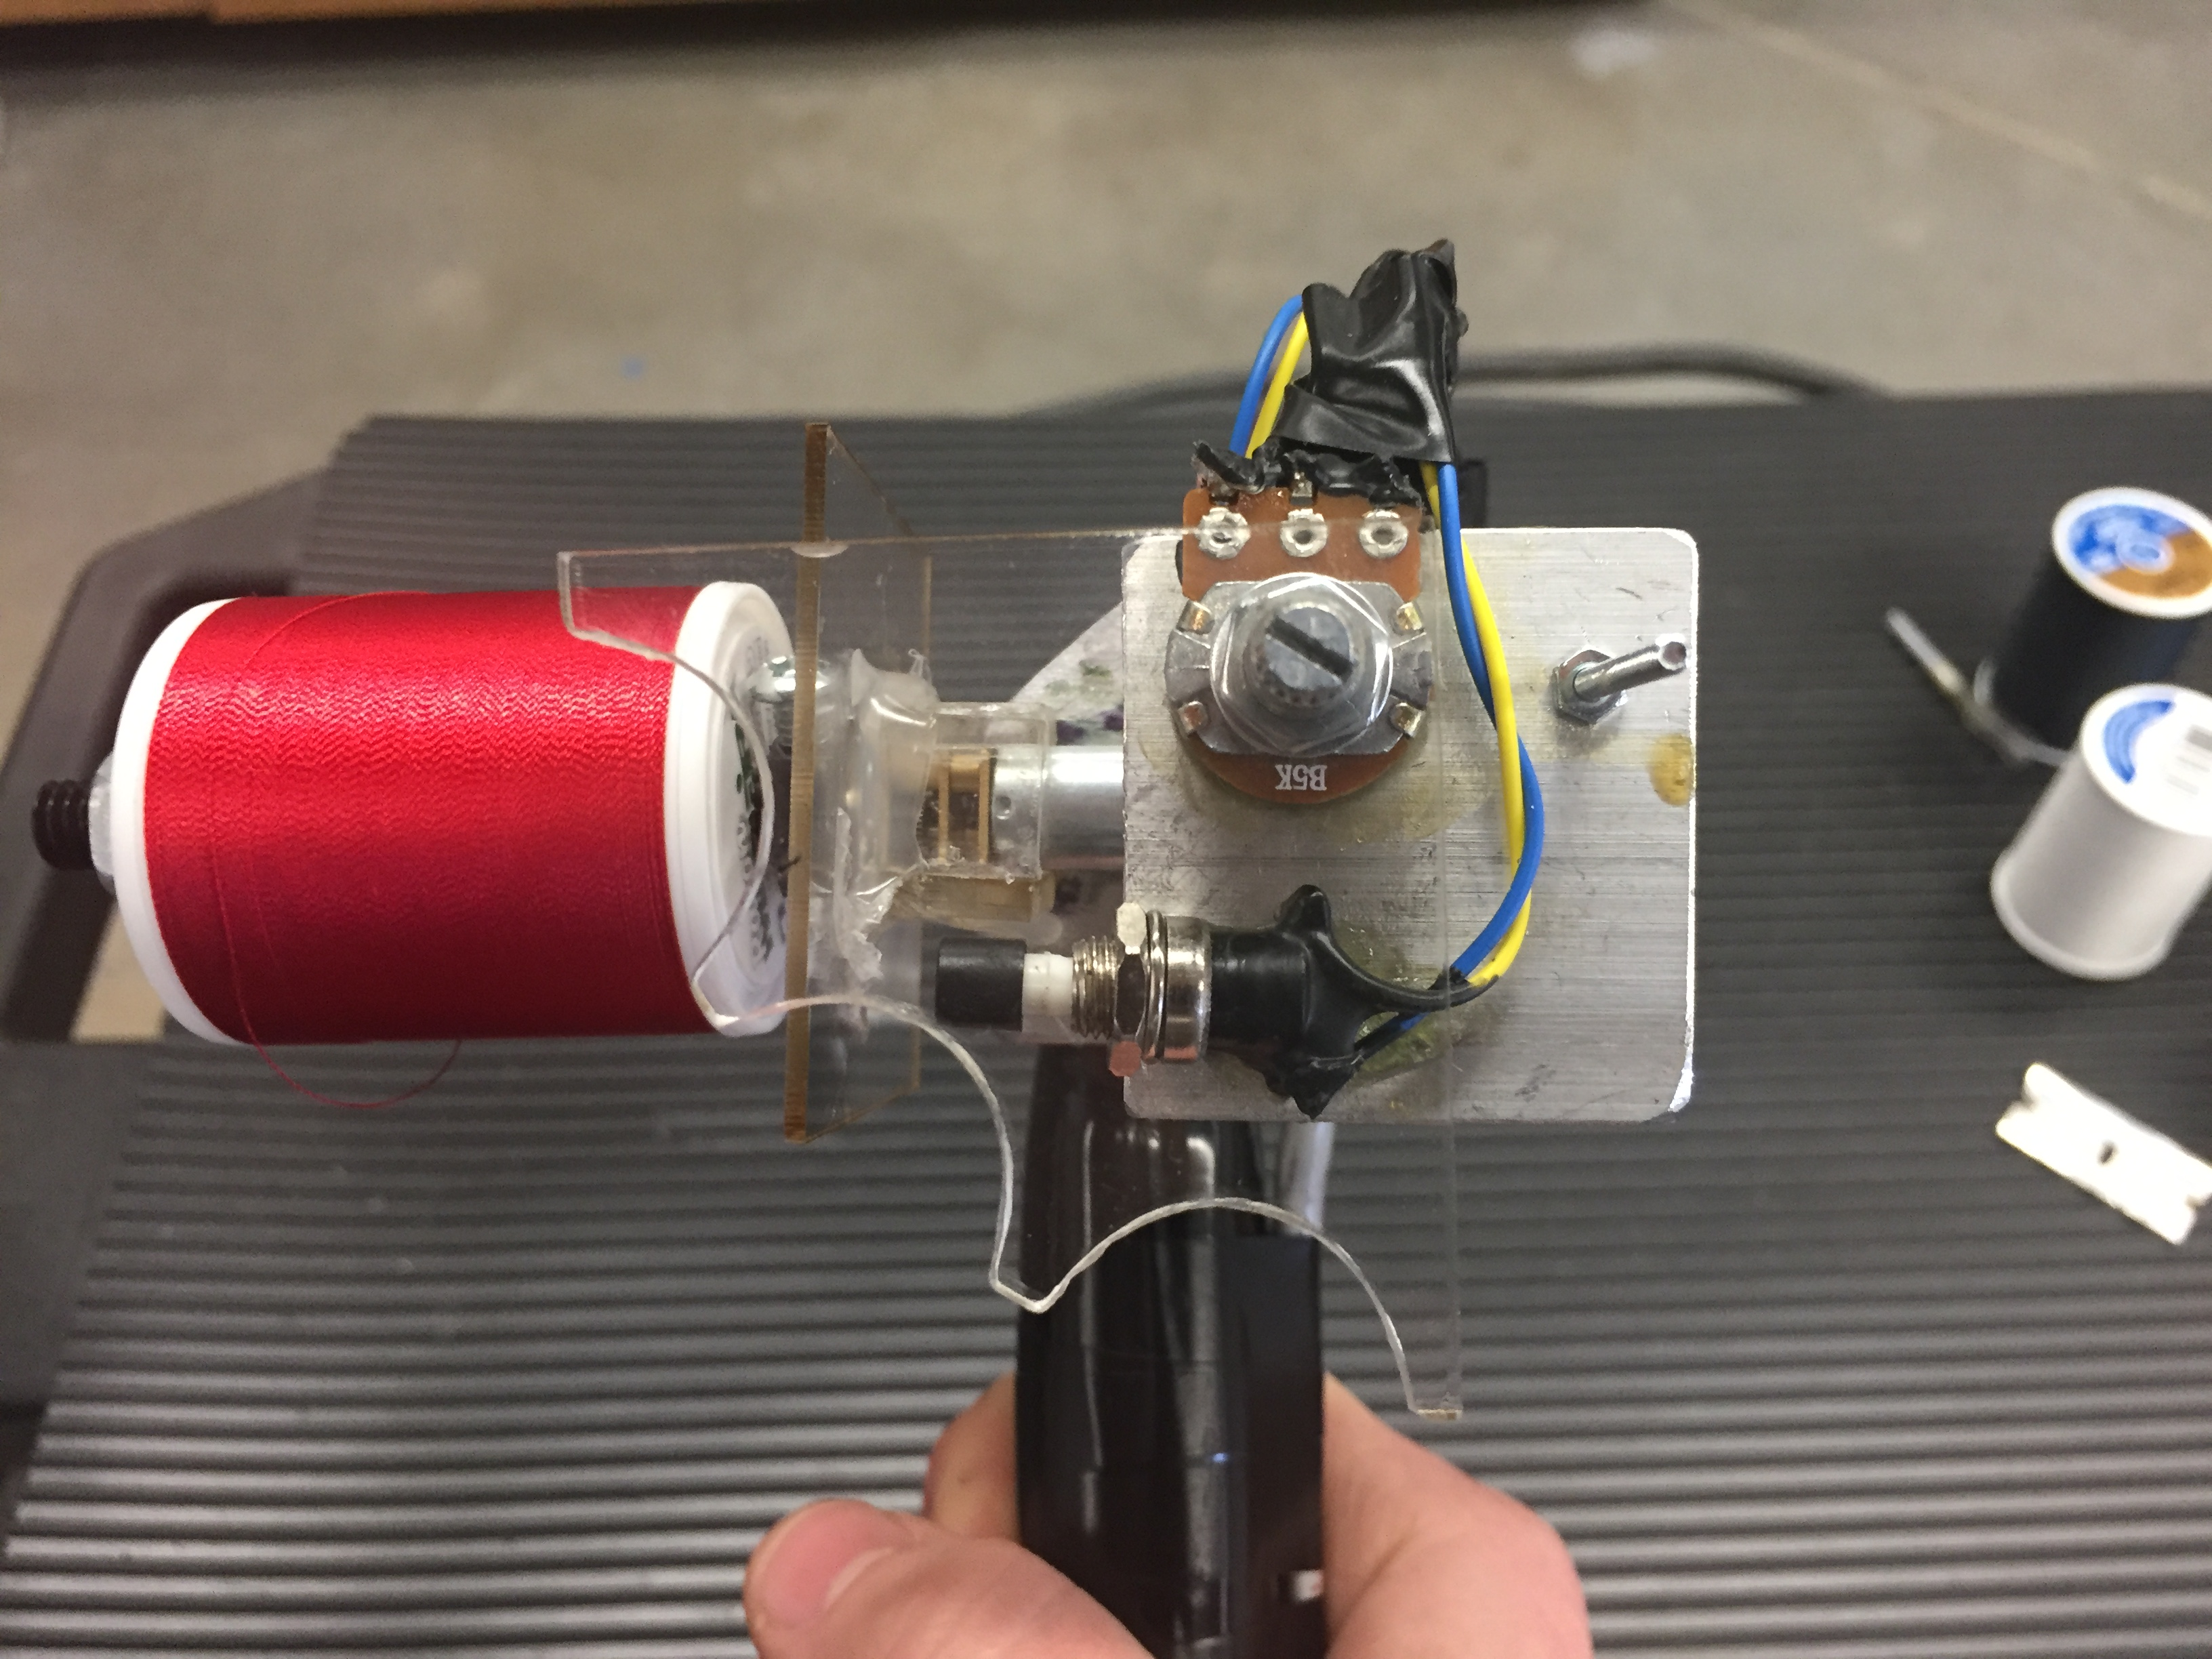
\includegraphics[width=0.9\linewidth]{controls_off.jpg}
\end{subfigure}%
\begin{subfigure}{.5\textwidth}
  \centering
  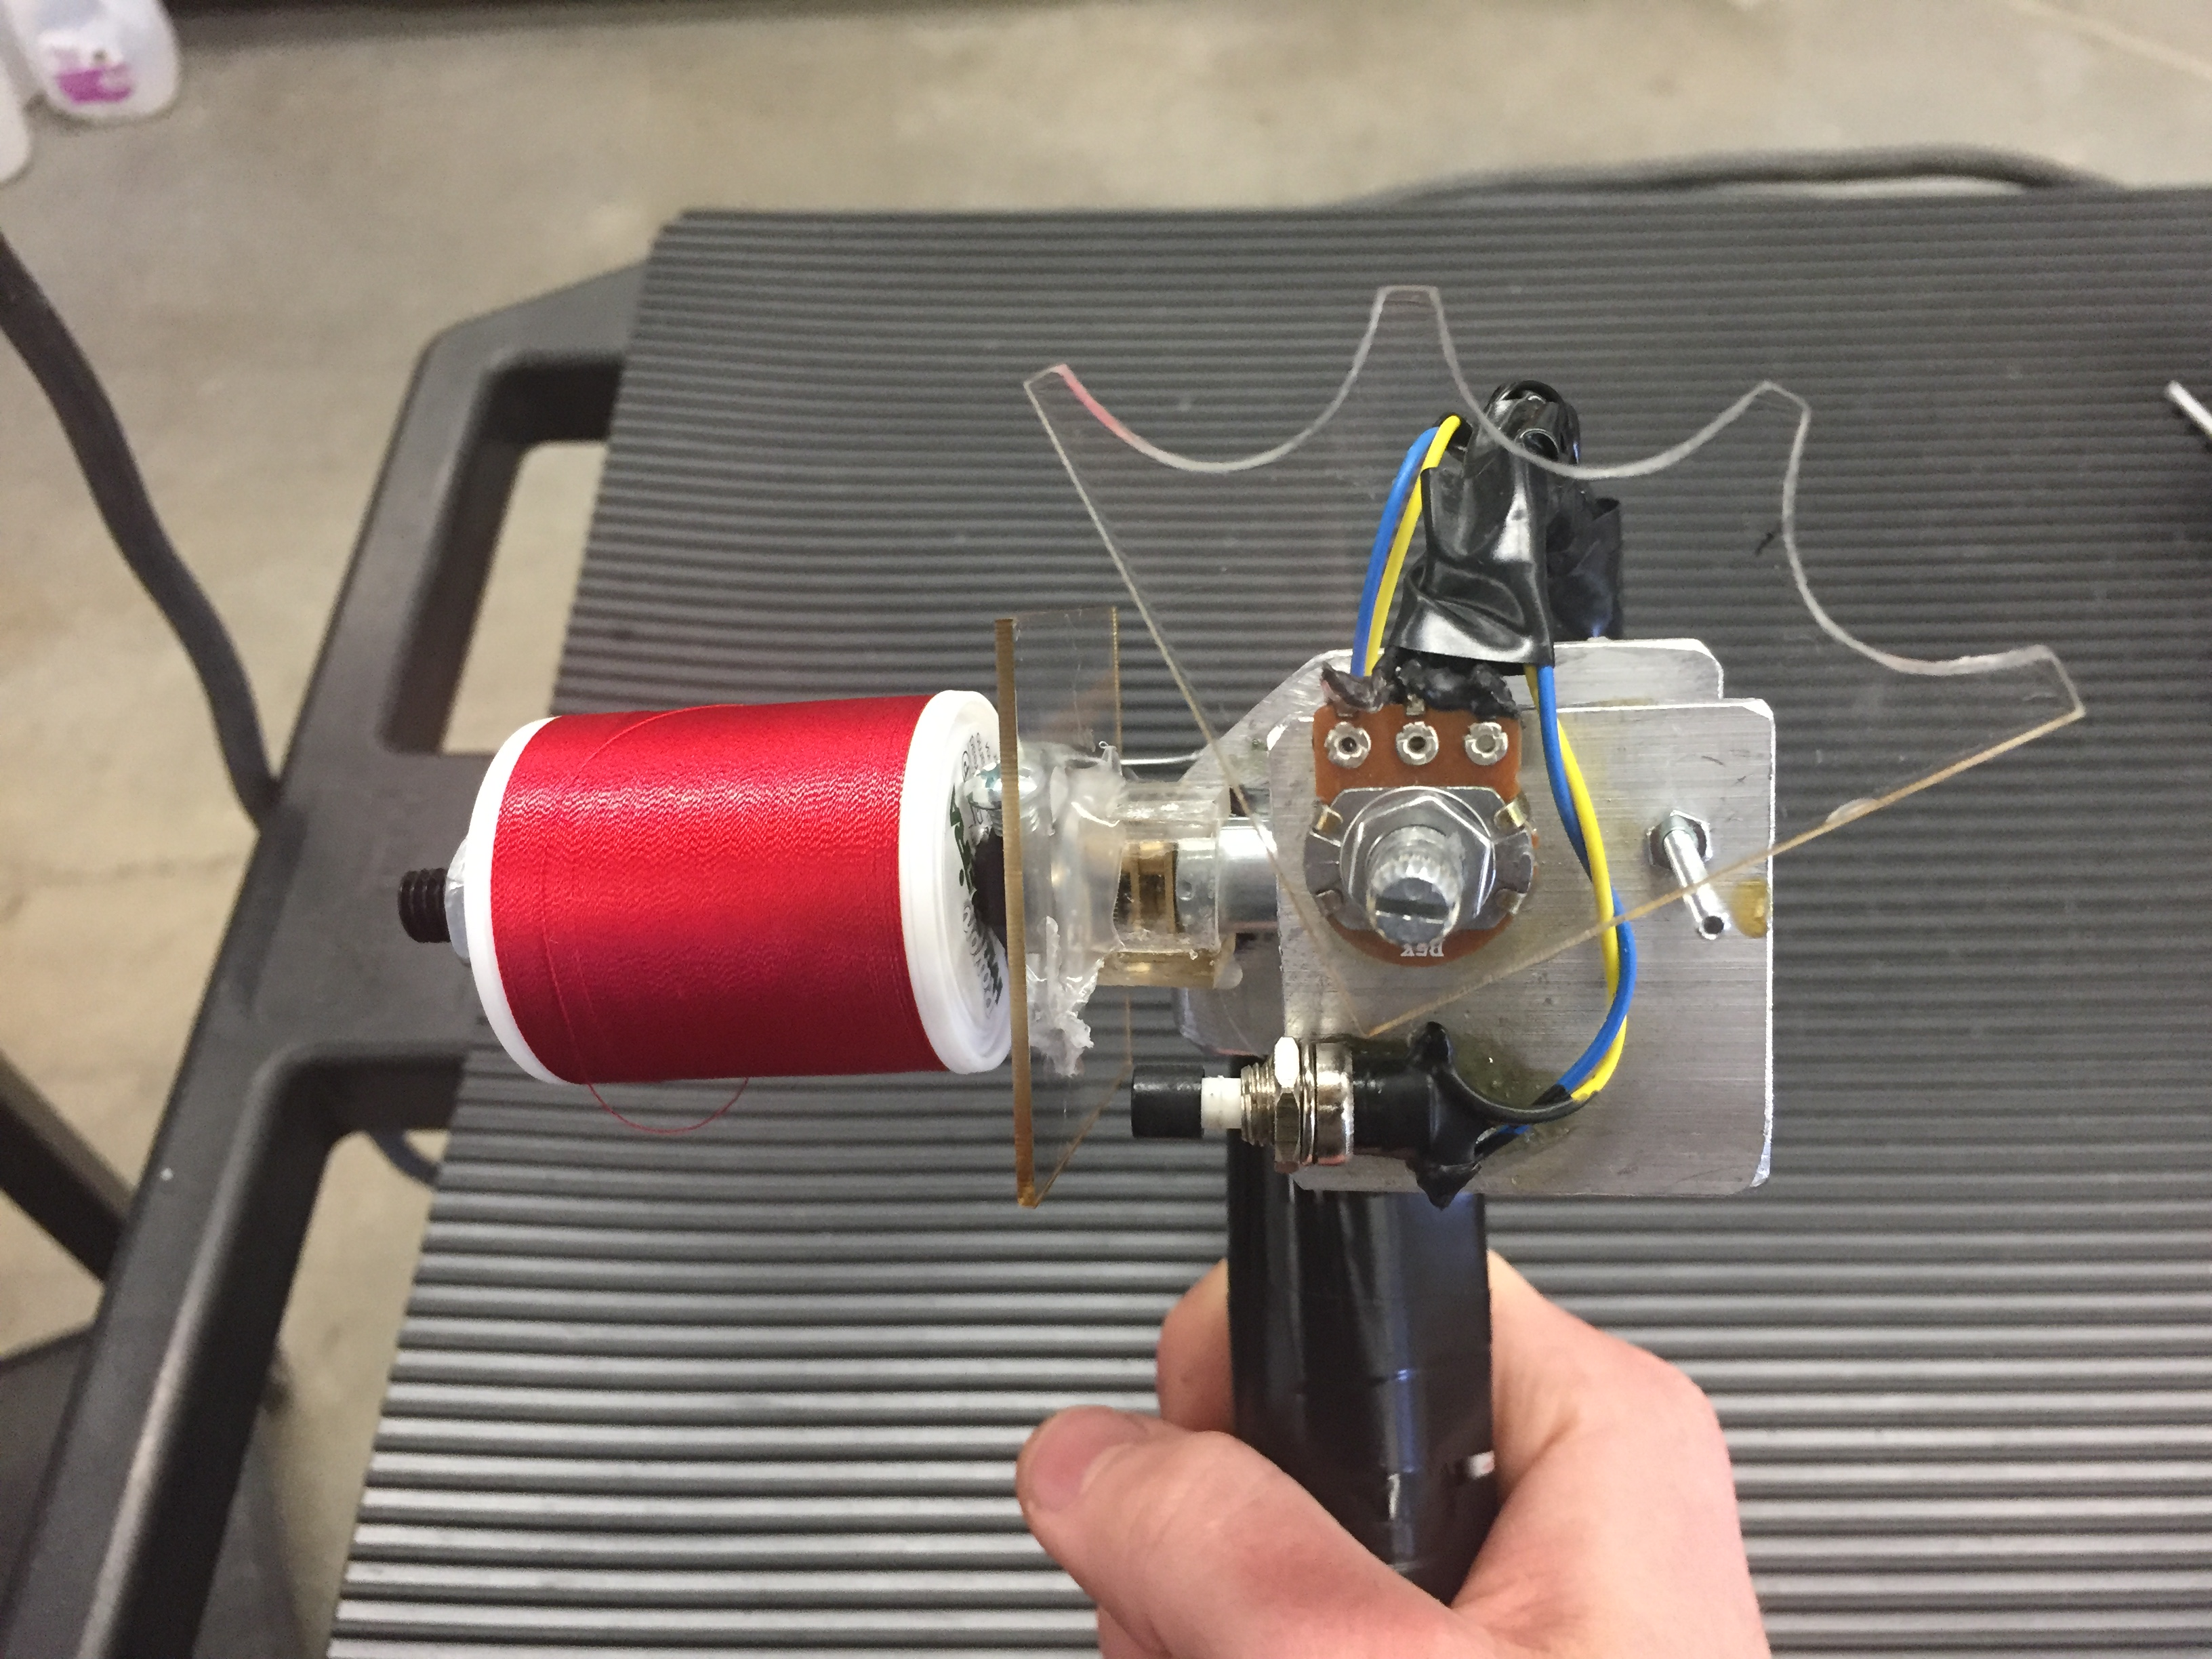
\includegraphics[width=0.9\linewidth]{controls_on.jpg}
\end{subfigure}
\caption{Position of speed control wheel (mounted on a potentiometer) when the motor is off (left) and at full speed (right). The motor reversal button is bottom-left to the speed control potentiometer.}
\label{fig:speed}
\end{figure}
Finally, make sure the thread is going through both the thread guide on the side of the gun and the through hole on the side of the permanent tip. To feed the thread into the through hole, push the thread near/into the through hole while blowing nitrogen through the gun. Here it is helpful to have a clean end of thread, so cut the thread with a razor or scissors if necessary. The properly threaded gun is shown in figure~\ref{fig:start_thread}. \par
\begin{figure} [h!]
		\centering
		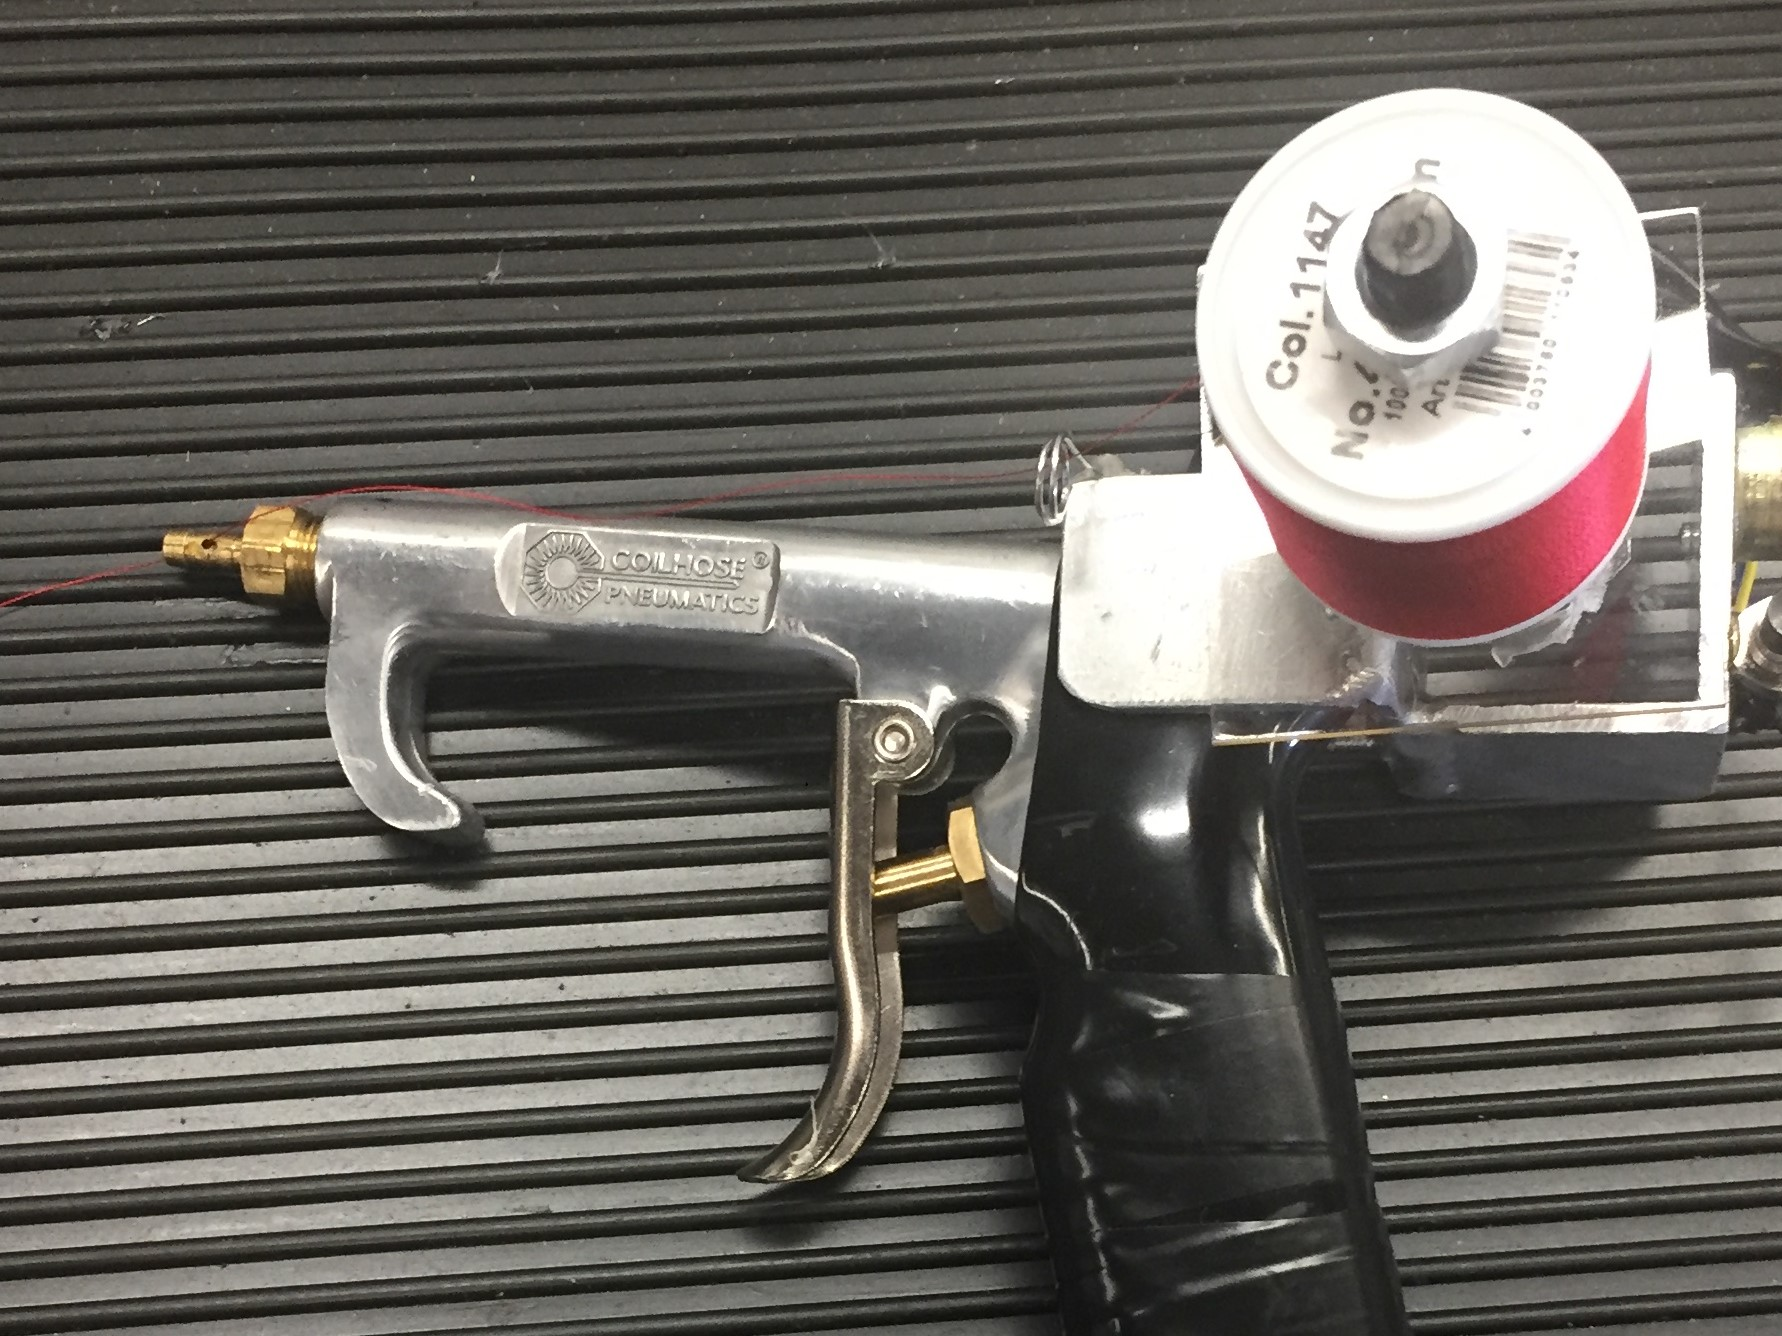
\includegraphics[width=0.75\textwidth]{gun_thread_up_zoom.JPG}
		\caption{Gun with thread in place. The thread guide (bent paperclip) is immediately to the left of the spool.}
		\label{fig:start_thread}
\end{figure}

\subsection{Threading Straws}
The process of threading straws is all dependent on angle and distance to the straw, and steadiness of hand. Future developments of the tip design (as described in the Future Upgrades section) will aim to make this process more forgiving. With the thread gun set up and less than 1cm thread sticking out of the tip, get into position in front of the desired straw as shown in figure~\ref{fig:no_tip}. The thread sticking out of the gun is inserted into the straw. While standing, the natural angle that most people hold the gun at is within this desired angular range. Once in place, start by squeezing the trigger to blow nitrogen through the straw. If this causes the thread to blow out of the straw, adjust the gun position and try again.\par
\begin{figure} [h!]
		\centering
		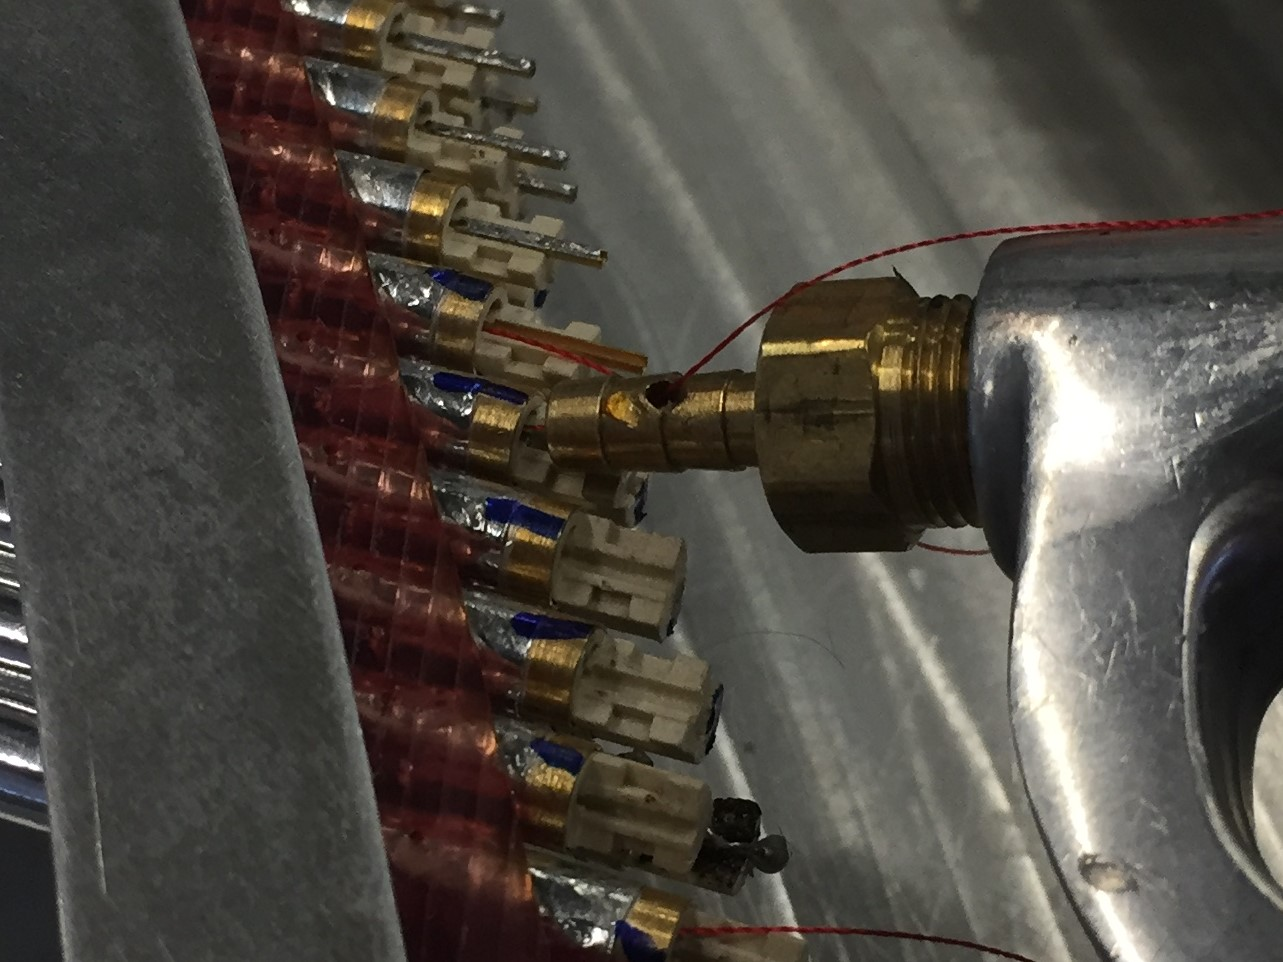
\includegraphics[width=1\textwidth,angle=0]{no_tip_zoom.JPG}
		\caption{Approximate gun positioning for threading straws. Tip can rest on top of the vectra and should have an angle such that the nitrogen blows down and into the straw.}
		\label{fig:no_tip}
\end{figure}
Now, with the nitrogen flowing, slowly adjust the speed control wheel to let out 2-3" of thread. Again, if the thread blows out of the straw, adjust the tip position and try again. Once a few inches of thread are in the straw, the speed can be increased. At full speed, the nitrogen at 10psi should still be able to propel the thread through the straw without getting tangled. Once the thread emerges from the opposite end of the straw, allow approx. 6" of thread to blow out of the far end of the straw. Turn off the motor and release the trigger. Slowly let out a few more inches of thread as the thread gun is pulled away from the straws. Again turn the motor off and cut the thread near the tip of the gun using a razor blade or scissors. If after 10-15 seconds the thread has not emerged from the straw, turn off the motor and release the trigger. Remove the tip from the straw and cut the thread. After pulling the likely bunched thread out of the straw, try again. 

\subsection{Cleanup \& Storage}
When the threader is not in use, turn off the electronics box (silver toggle switch). Additionally, turn off the nitrogen supply. During everyday use, this can be accomplished by simply turning the valve on the nitrogen tank clockwise until tight. If desired, the second valve can also be closed now. Properly dispose of any thread in the garbage and return the gun and cart the designated location in the lab.


\section{Cost Analysis} \textbf{Total Cost Estimate: \large{\$154.89}} \\ \\
Note: Each component is hyperlinked to a relevant web page to purchase from.
\subsection{Gun Components: Subtotal \$56.07}
\begin{itemize}
\item{\href{https://www.amazon.com/Milton-S-160-Pistol-Grip-Blow/dp/B00HFL7OYC/ref=sr_1_38?ie=UTF8&qid=1502990735&sr=8-38&keywords=air+blowgun}{Pistol grip blow gun}, \$15.41
}
\item{Aluminum motor \& control mount with set screws, \$10? (see Nathaniel Pearson, machining these components in house)
}
\item{\href{https://www.grainger.com/product/8AT33?cm_mmc=PPC:+Google+PLA&s_kwcid=AL!2966!3!57772102677!!!g!109228327077!&ef_id=WiAW8AAABCj3Xkj0:20180131221551:s&kwid=productads-adid^57772102677-device^c-plaid^109228327077-sku^8AT33-adType^PLA}{Plastic tubing 1/8" ID, 1/4" OD (15')}, \$6.30 (\$18.90 for 50' length, good for 3 guns)
}
\item{\href{https://www.digikey.com/product-detail/en/assmann-wsw-components/A-MO-8-8-F50/AE10316-ND/1957592}{RJ45 plug}, \$0.36
}
\item{\href{https://www.amazon.com/Mediabridge-Ethernet-Cable-Feet-Networking/dp/B001W26TIW/ref=pd_sbs_147_2?_encoding=UTF8&pd_rd_i=B001W26TIW&pd_rd_r=CBZP87PN82231S59BQCK&pd_rd_w=6axY9&pd_rd_wg=DrKOm&psc=1&refRID=CBZP87PN82231S59BQCK}{CAT5 cable, stranded (15')}, \$3.17 (\$9.48 for 50' length, good for 3 guns)
}
\item{\href{https://www.amazon.com/uxcell-100RPM-Reduction-Terminals-Engine/dp/B0711MPZ64/ref=sr_1_8?s=hi&ie=UTF8&qid=1516662559&sr=1-8&keywords=100rpm\%2Bdc\%2Bmotor&th=1}{DC 12V 100RPM motor}, \$8.73
}
\item{\href{https://www.digikey.com/product-detail/en/precision-electronics-corporation/RV4NAYSD502A/RV4N502C-ND/222807&?gclid=EAIaIQobChMI99OA4qOD2QIVFbjACh3Cfg-0EAQYAiABEgKr0PD_BwE}{5k Potentiometer (speed control)}, \$9.77
}
\item{\href{https://www.digikey.com/product-detail/en/te-connectivity-alcoswitch/MSPS103C0/450-1664-ND/529502&?gclid=EAIaIQobChMI6vDSpsaC2QIVRLnACh3oGw7aEAQYASABEgK0UvD_BwE}{Pushbutton (motor reversal)}, \$2.33
}
\item{1/4" plastic bolt, set screw, and nut, unknown cost. See Nathaniel Pearson for more information. We currently have 3 completed sets of the bolt units.
}
\item{Custom Plexiglass speed control wheel (as seen in figure~\ref{fig:speed}), free (laser cut by Mitch Frand)
}
\item{\href{https://www.amazon.com/Madeira-9841-1147-Rayon-Embroidery-Thread/dp/B004KYZF9I}{Madeira 9841 - 1147 Rayon Embroidery Thread, 40wt/1100 yd}
}
\end{itemize}

\subsection{Electronics Box: Subtotal \$98.82}
Note: The current cost analysis and linked products are for the proposed PCB, not the current prototype box.
\begin{itemize}
\item{\href{https://www.amazon.com/gp/product/B01983R7PK/ref=oh_aui_detailpage_o03_s00?ie=UTF8&psc=1}{Arduino Nano}, \$9.99
}
\item{\href{https://www.pololu.com/product/1110}{Pololu Qik 2s9v1 dual serial motor controller}, \$24.95
}
\item{\href{https://www.pcbgogo.com/orderonline.aspx}{Printed Circuit Board}, \textasciitilde\$5 (5 or 10 boards for \$5 + \$15-\$20 to ship from China)
}
\item{\href{https://www.digikey.com/product-detail/en/adafruit-industries-llc/85/1528-1074-ND/5154649?WT.srch=1&gclid=EAIaIQobChMItfGY14iD2QIVRJ7ACh3RtgqiEAYYAyABEgJZSvD_BwE}{Female header pins}, \$1.95 (might be a few headers short, but we have some extras in PAN 450)
}
\item{\href{https://www.digikey.com/product-detail/en/stackpole-electronics-inc/RNMF14FTC6K20/S6.2KCACT-ND/2617529}{Resistor (pull up resistor for button)}, \$0.10 (we probably have some of these in PAN 385)
}
\item{\href{https://www.digikey.com/product-detail/en/tdk-corporation/CK45-B3AD222KYNNA/445-16006-ND/4457608}{2.2nF Capacitor}, \$0.37
}
\item{\href{https://www.digikey.com/product-detail/en/e-switch/100SP1T1B1M1QEH/EG2350-ND/378819}{Toggle switch (power)}, \$2.11
}
\item{\href{https://www.digikey.com/product-detail/en/cinch-connectivity-solutions-johnson/108-0902-001/J151-ND/5929}{Banana jack, red (+12V)}, \$0.65
}
\item{\href{https://www.digikey.com/product-detail/en/cinch-connectivity-solutions-johnson/108-0903-001/J152-ND/5930}{Banana jack, black (GND)}, \$0.65
}
\item{\href{https://www.digikey.com/product-detail/en/amphenol-fci/54602-908LF/609-1046-ND/1001360}{RJ45 Jack (connect box to gun)}, \$0.60
}
\item{\href{https://www.amazon.com/ExpertPower-EXP12180-Rechargeable-Battery-Bolts/dp/B00A82A3RK/ref=pd_rhf_dp_s_cp_0_1?_encoding=UTF8&pd_rd_i=B00A82A3RK&pd_rd_r=AV6KKGY30GWW44717RG1&pd_rd_w=rgVh3&pd_rd_wg=pwAHe&refRID=AV6KKGY30GWW44717RG1&th=1}{12V 18Ah rechargable sealed lead acid battery (AGM Tech)}, \$33.99
}
\item{\href{https://www.amazon.com/Alligator-Pop-Time-Approved-Qualified/dp/B01IGSDSF6/ref=sr_1_9?ie=UTF8&qid=1516318913&sr=8-9&keywords=12v+battery+clips}{12V 1500mA sealed lead acid battery charger}, \$14.99
}
\item{\href{https://www.amazon.com/Test-Cable-TOOGOO-Alligator-Multimeter/dp/B01GO4PZDW/ref=sr_1_5?ie=UTF8&qid=1517497220&sr=8-5&keywords=banana+plugs+alligator+clips}{Banana plug/alligator clip power cables (1m)}, \$3.47
}
\item{Electronics box, free (scrounge in scrap electronic bins in PAN or talk to Mitch about laser cutting plexiglass enclosure)
}
\item{Electronics box front plate, free (laser cut plexiglass, see Mitch)
}
\end{itemize}


\section{Gun Assembly}
DP-810 epoxy was used to secure the motor and other electronics onto the mount, but it would be much simpler and more effective to drill holes into the aluminum mount to properly mount the components (except the motor). The motor mount could be adjusted such that the motor screws into the mount on the side of the motor shaft (there are two small mounting screw holes on the motor). Once the components are physically attached to the motor mount, solder the CAT5 cable to the components. When doing this, use heat shrink tubing on any solder joints where two wires are soldered together. With everything soldered in place, crimp on a RJ45 plug to the unused end of the cable. Use the wiring scheme designated in the Circuit Assembly section. After soldering everything in place, tidy up the gun wiring with electrical tape and liquid electrical tape. The CAT5 cable should be secured to the grip of the gun using electrical tape. This is shown in figure~\ref{fig:gun_wire}. Similarly, the cable and the gas tubing are tied together using electrical tape approx. every 1' along the wire/tube. Refer back to figure~\ref{fig:speed} for a good view of where the electronic components are positioned on the back of the gun.
\begin{figure} [h!]
		\centering
		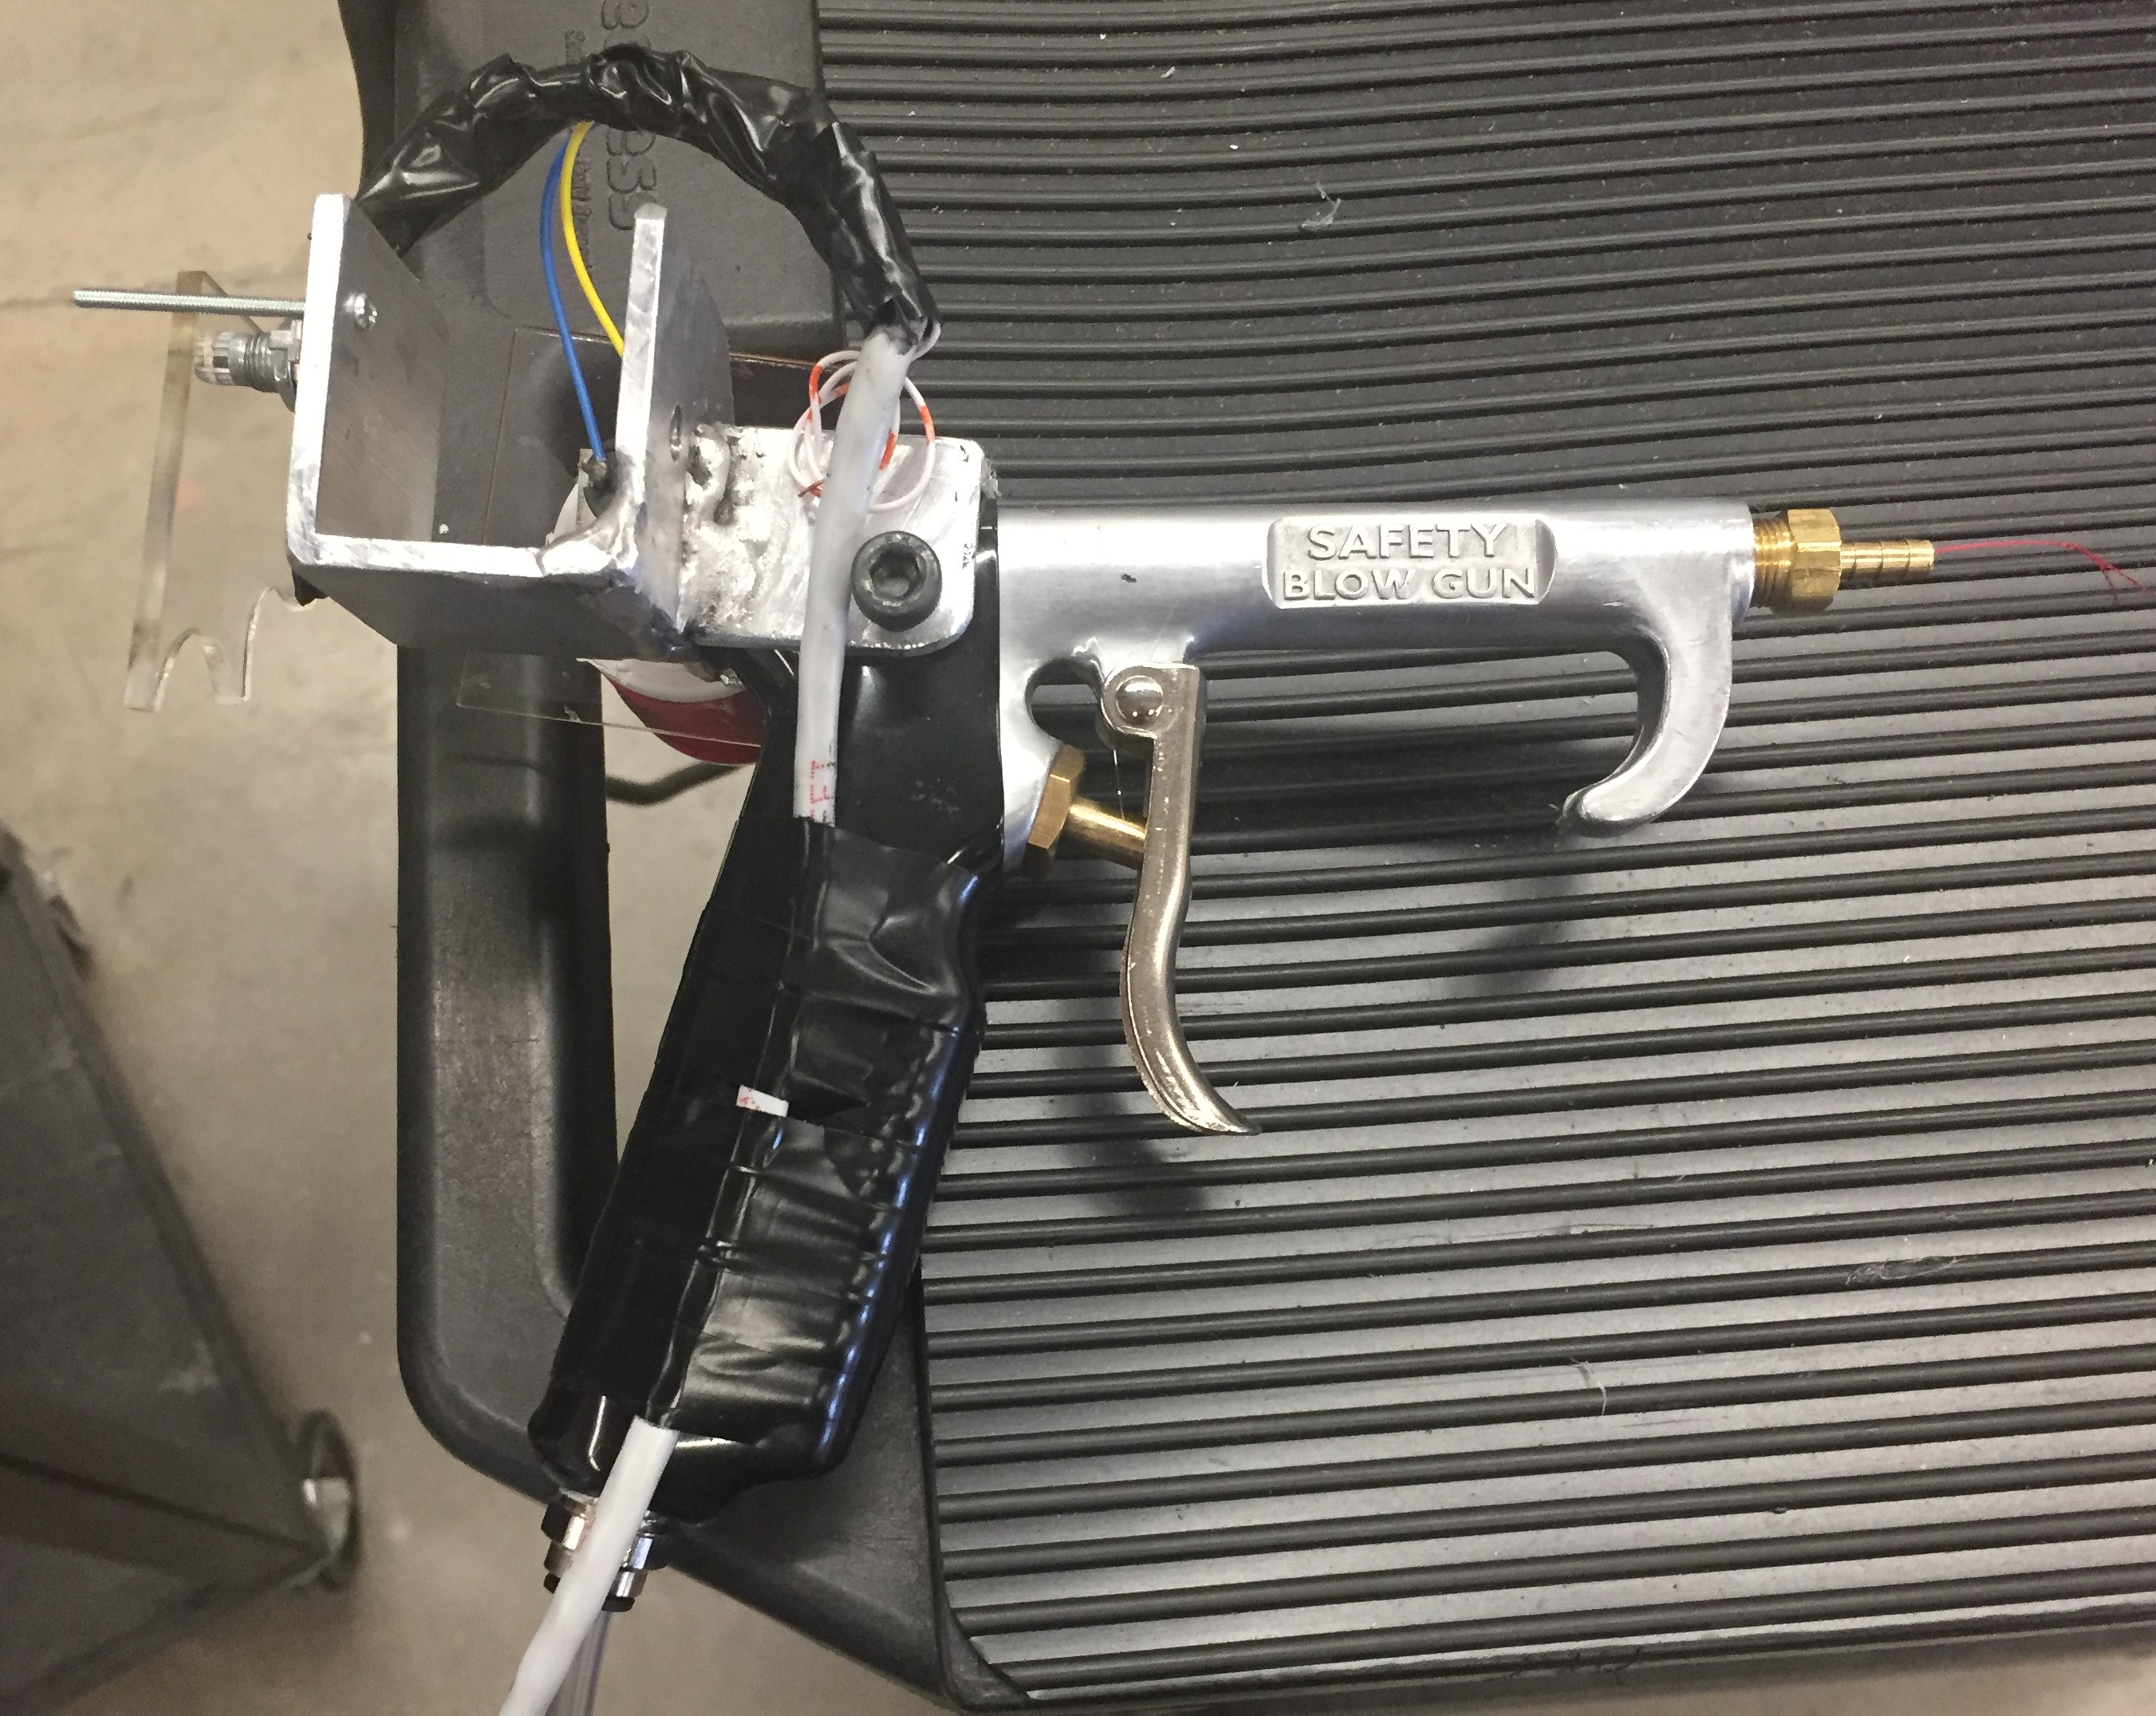
\includegraphics[width=0.75\textwidth]{gun_thread_down.JPG}
		\caption{The CAT5 cable is secured to the pistol grip using electrical tape. Leading out of the gun}
		\label{fig:gun_wire}
\end{figure}


\section{Circuit Assembly}
The prototype circuit was soldered onto a cheap prototyping breadboard and fixed into the plastic box from a discarded ethernet switch (see figure~\ref{fig:box_innards}). In the future, if PCBs are designed, creation of laser cut plexiglass boxes should be considered. The next version of the electronics box should utilize female header pins so that the Arduino and Pololu can be swapped out if any components fail. A schematic of the current electronics box circuit and gun electronics is attached on the following page.
\begin{figure} [h!]
		\centering
		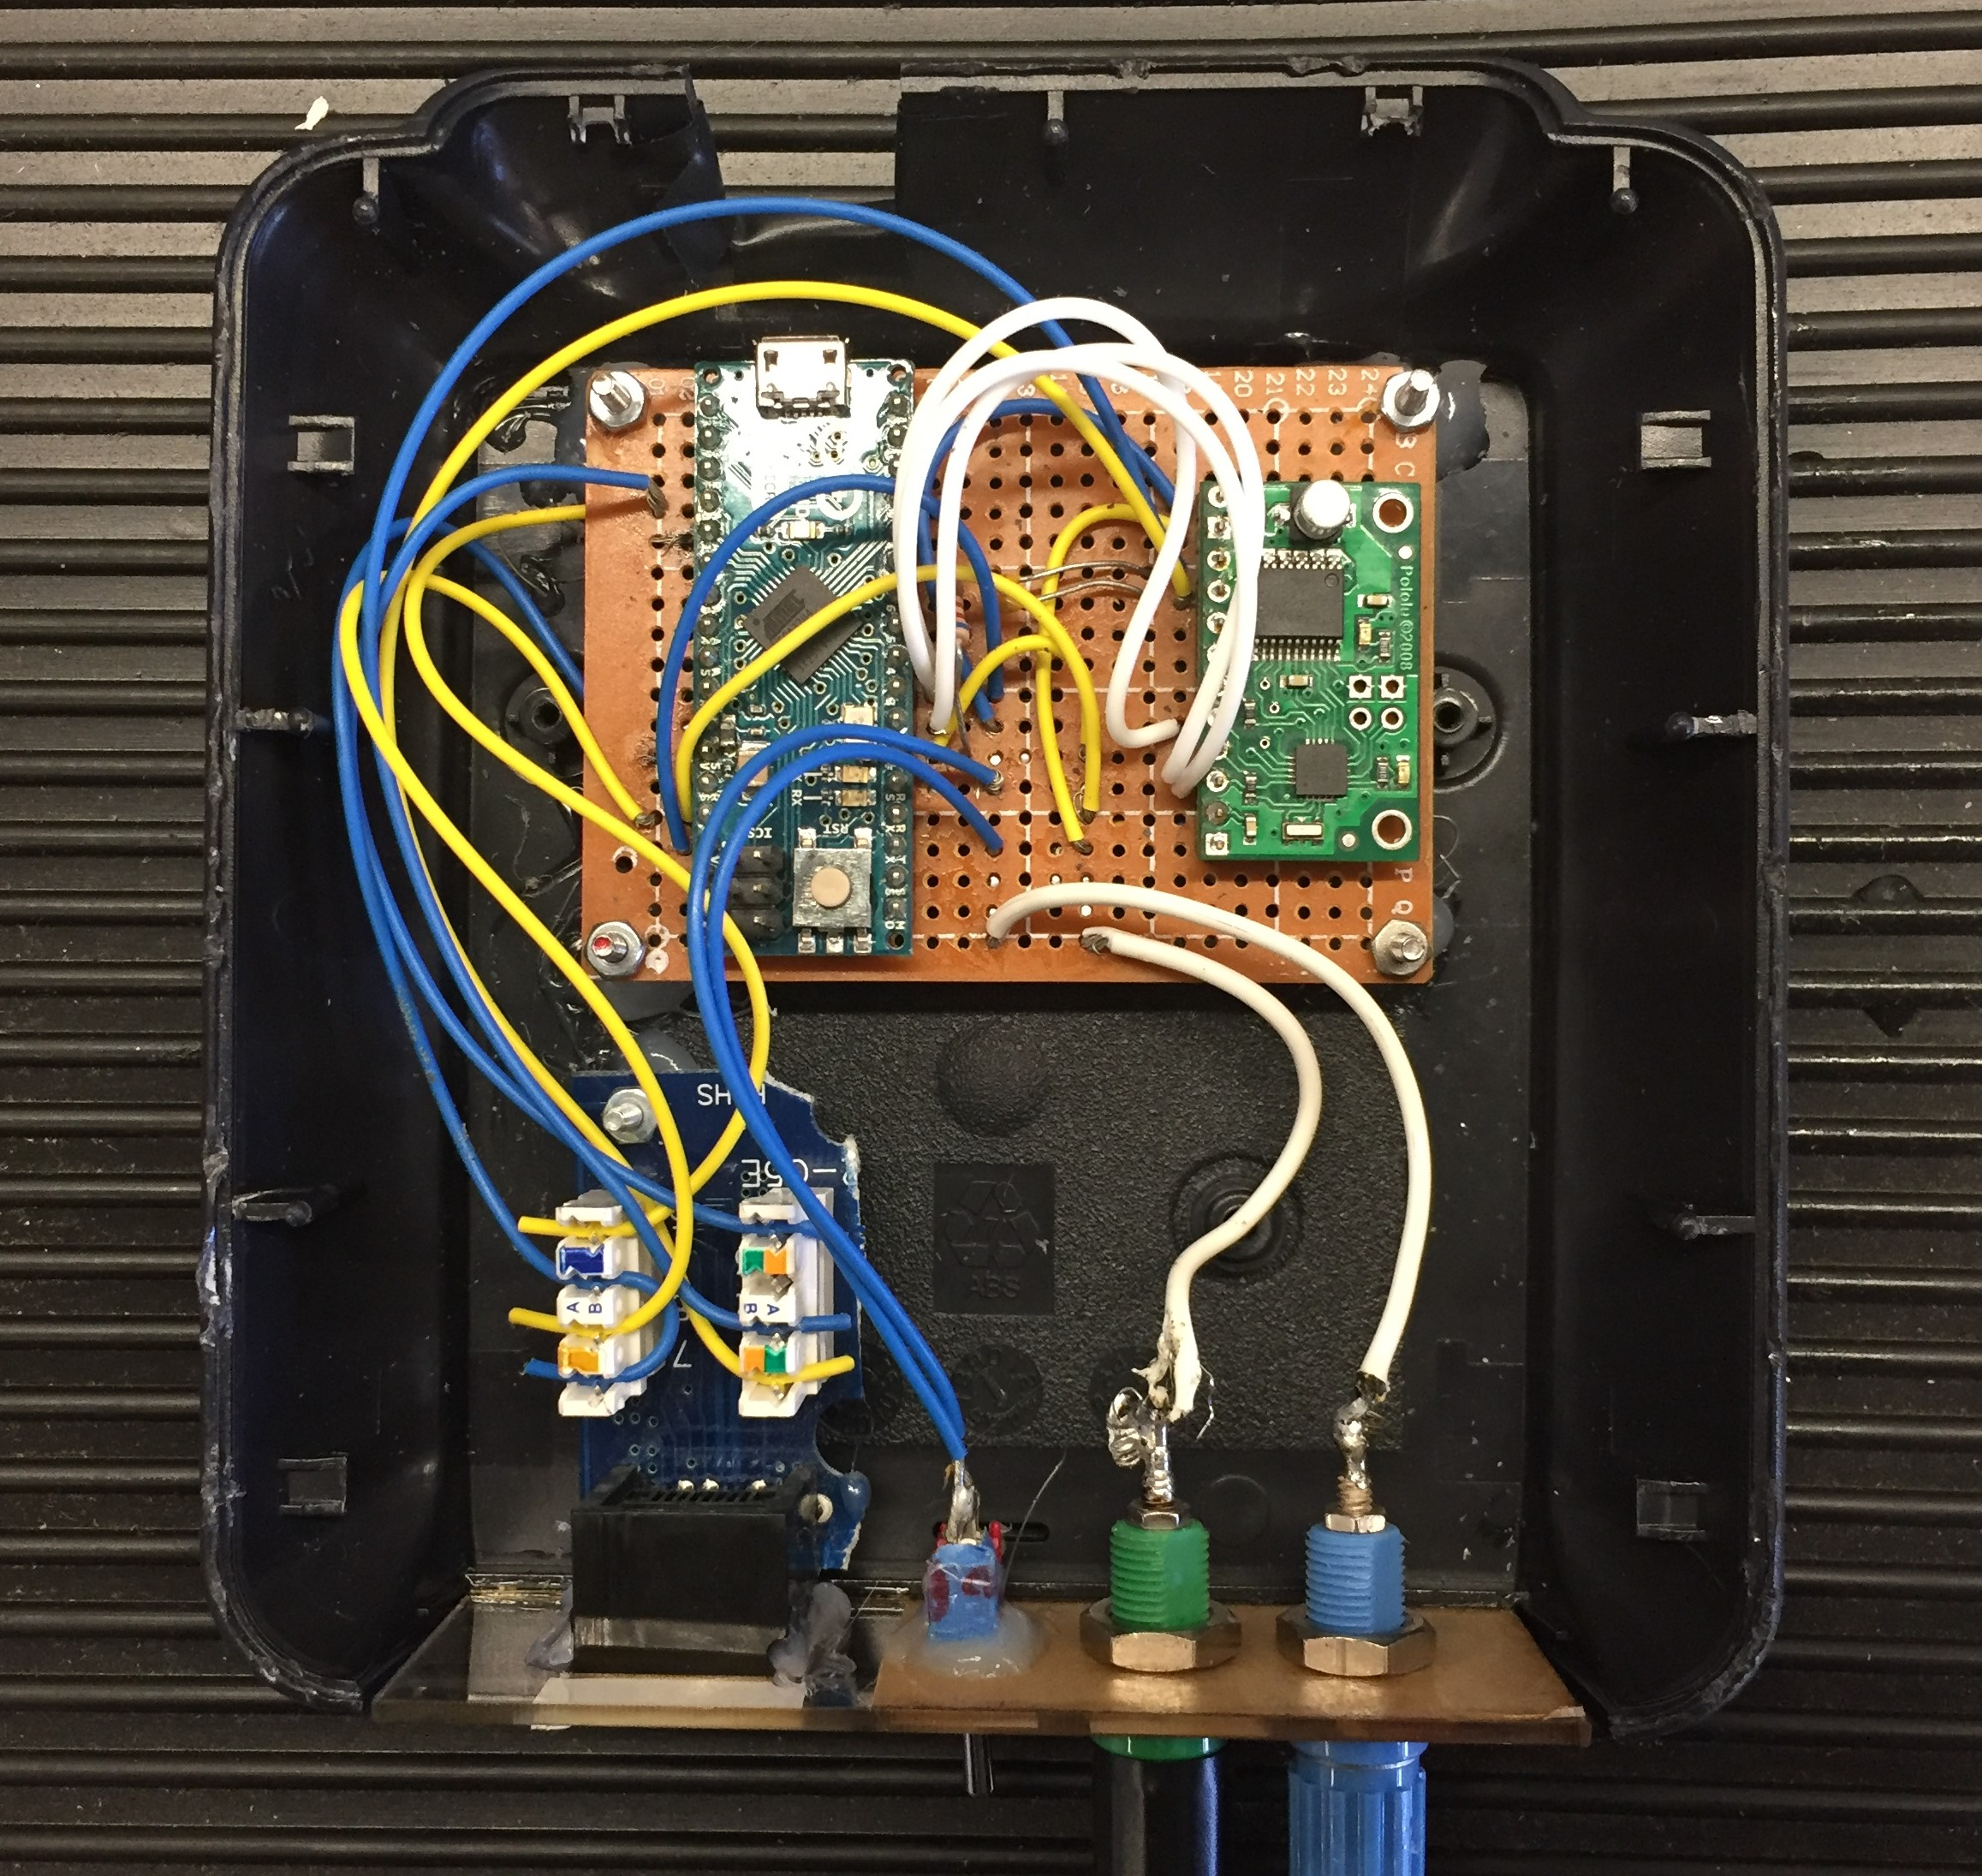
\includegraphics[width=0.8\textwidth]{electronics.JPG}
		\caption{The prototype circuit fitted in the recycled electronics case. A small hole is routed in the box (top of image) so the USB port of the Arduino is accessible from the exterior of the box.}
		\label{fig:box_innards}
\end{figure}
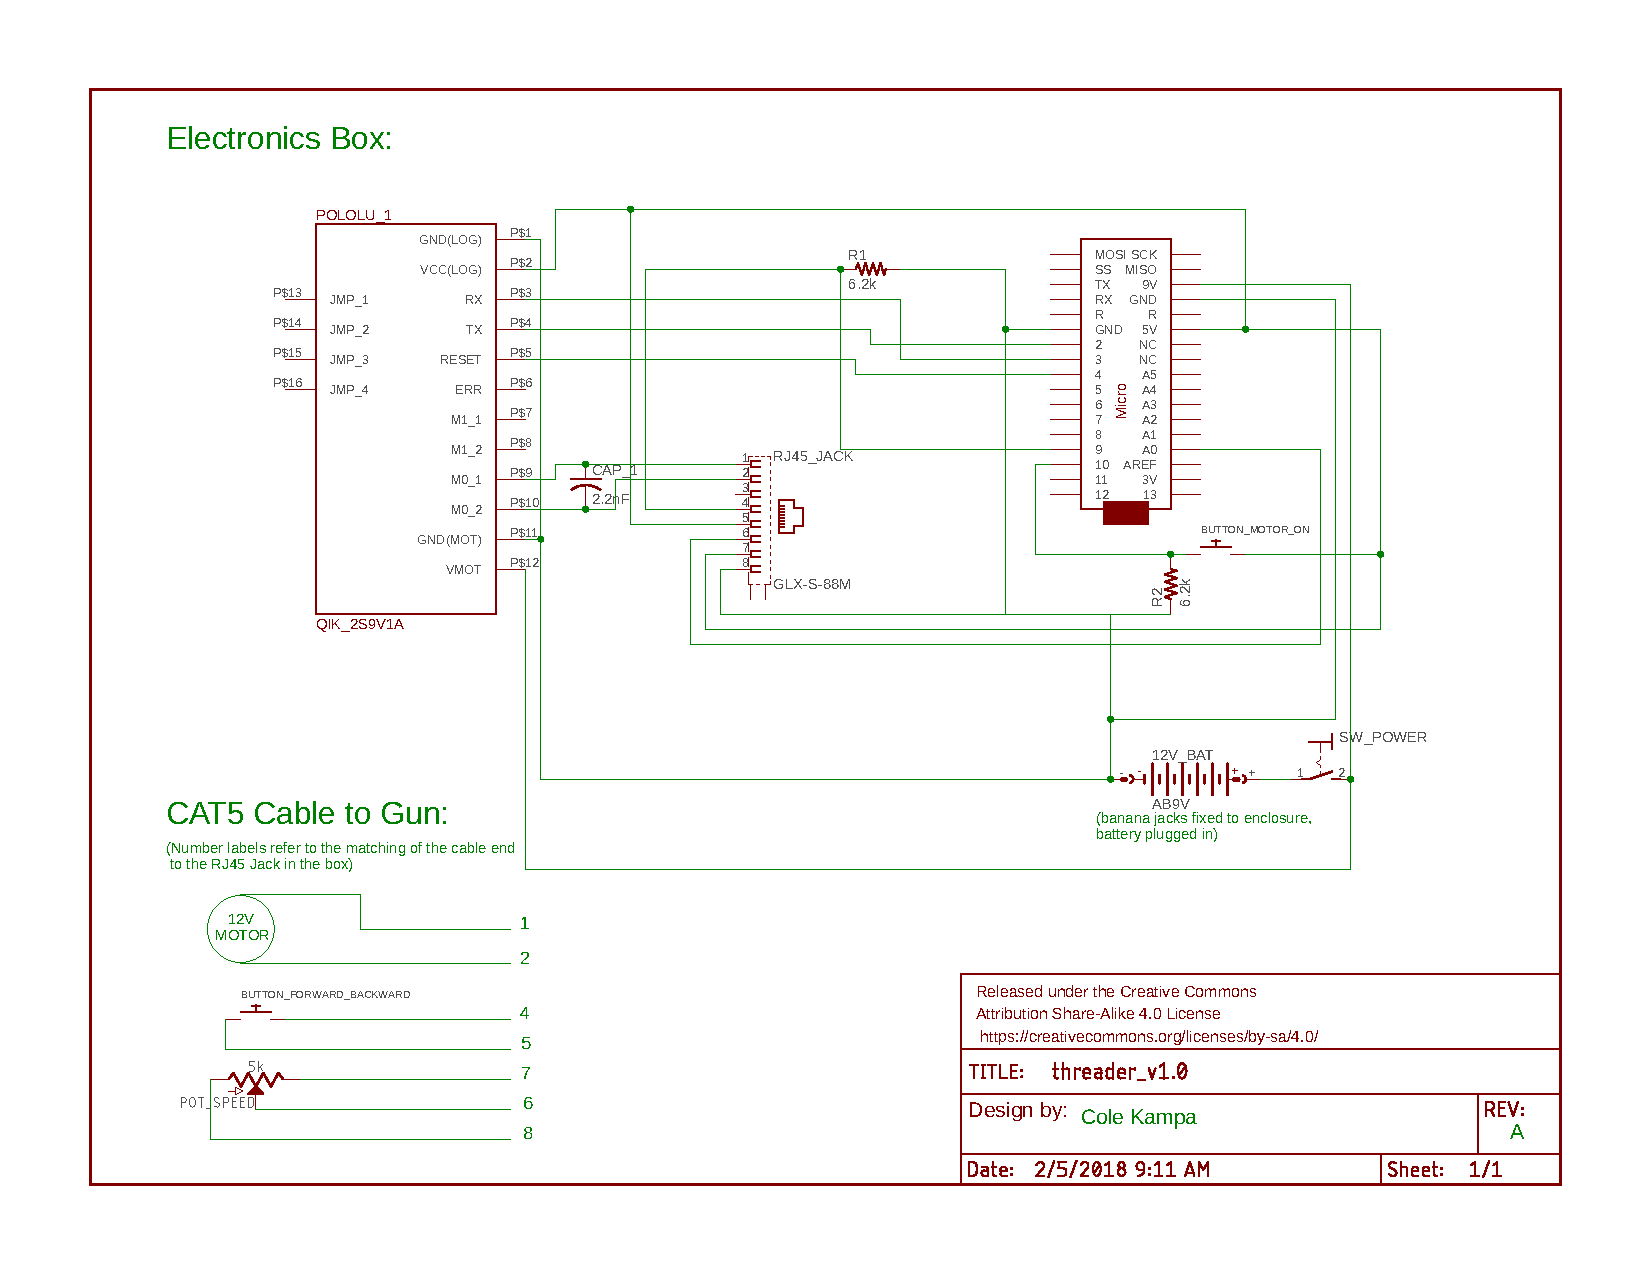
\includepdf[angle = 90, pagecommand={},scale=0.82475]{threader_circuit_v1_0.pdf}


\section{Future Upgrades}
\begin{itemize}
\item{
\textbf{Nitrogen on cart:} To make the cart fully mobile, we aim to find an easy way to put a smaller nitrogen tank on the bottom shelf of each cart. See Jason Bono for progress updates here.
}
\item{
\textbf{Nozzle design:} The most effective tip design has yet to be determined. Currently, three tips are being tested (no added tip, nesting tip, flat tip).
}
\item{
\textbf{Spool fins:} One problem with the current design is that thread falling behind the spool causes a halt in operating the gun. This problem is particularly prevalent with full spools, as the thread often falls off due to gravity and a lack of tension. The current idea is to add fins or some other enclosure behind the spool to prevent this from happening. Some initial prototyping was done with the spool itself and the gun. On the spool, small tabs of plexiglass were attached using hot glue to act as fins. Additionally, a 'backboard' was added to the front of the motor. These are shown in figure~\ref{fig:fins}.
}
\begin{figure} [h!]
		\centering
		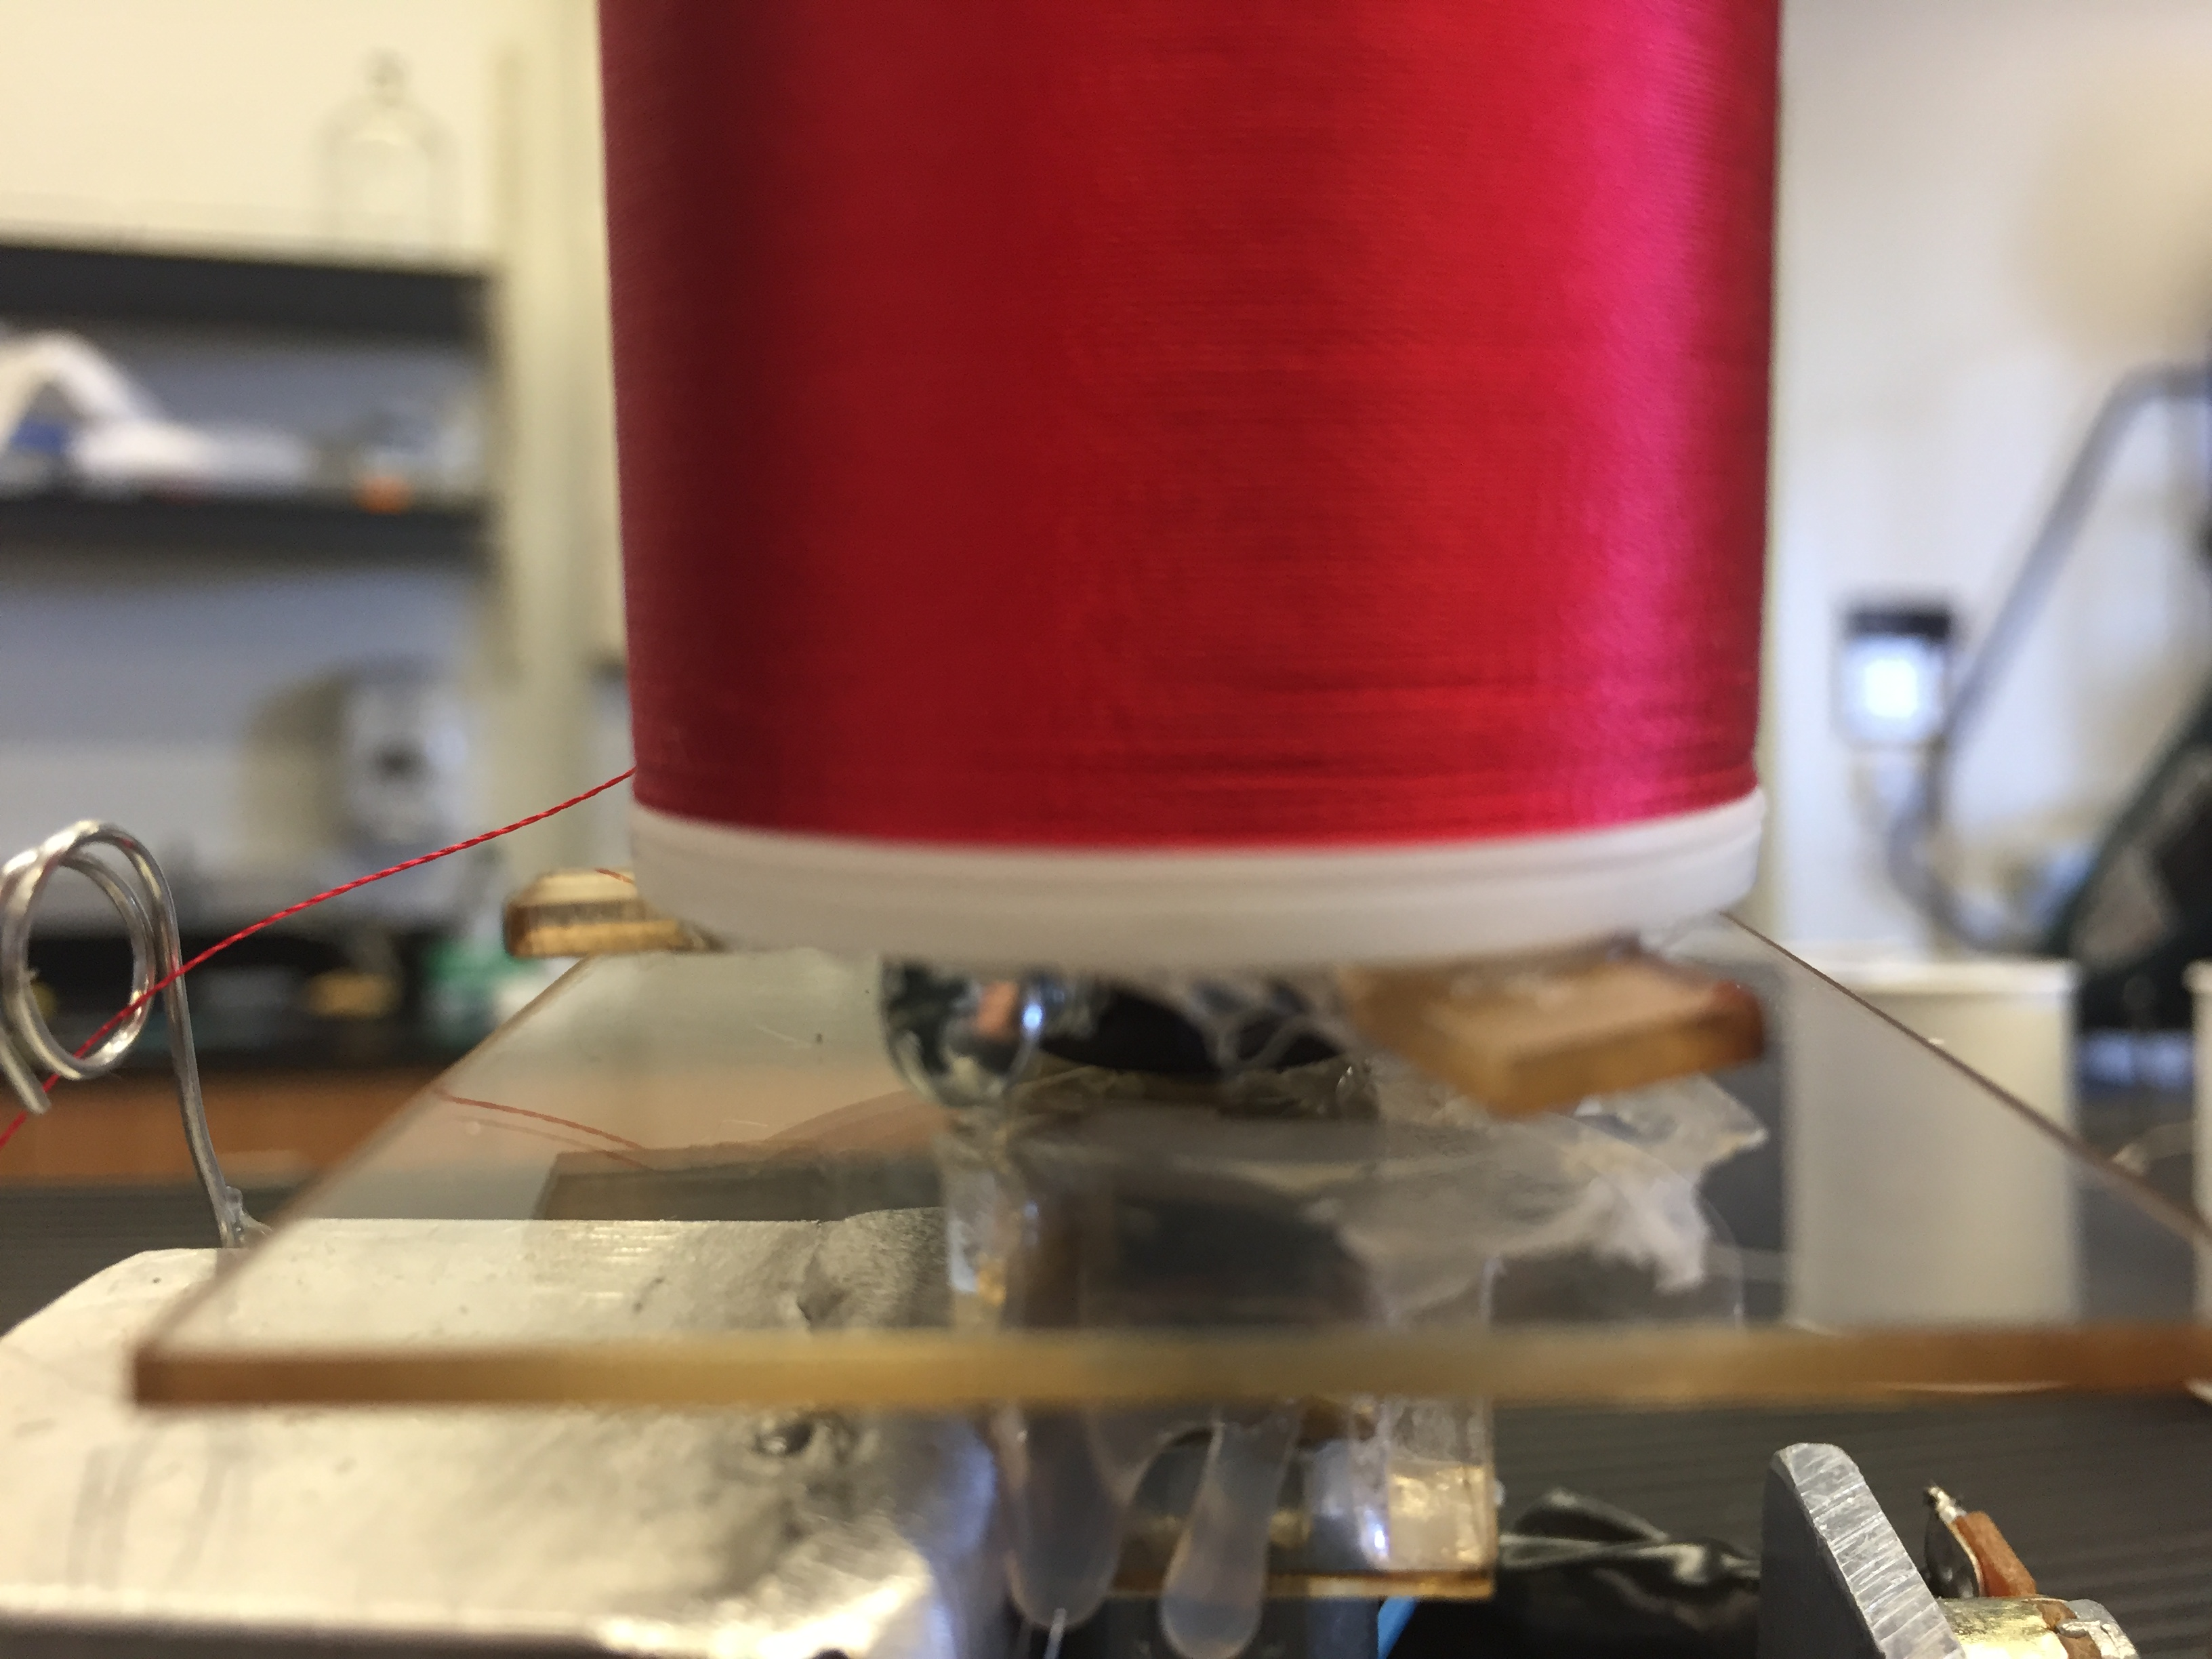
\includegraphics[width=0.9\textwidth]{fins_upgrade.JPG}
		\caption{Prototype fin system to prevent thread tangling and binding the gun.}
		\label{fig:fins}
\end{figure}
\item{
\textbf{Printed circuit board (PCB):} The design of a PCB should make the circuit much sturdier and should cut down assembly time significantly. We can also slightly decrease the circuit's footprint. Note again that we would prefer a design that implements female header pins so the Arduino and Pololu boards can easily be swapped if anything breaks. Costs for a PCB are included in the cost analysis above, but the actually PCB still needs to be designed.
}
\item{
\textbf{High/Low Speed Switch:} There have been some concerns with the decrease in thread speed as the spool runs low (linear function of radius of the thread). If this problems significantly slows down threading, a simple pole switch (or button) could be added to the circuit to toggle between high and low speed settings. The low speed should be calibrated to work with a full spool, while the high speed would be calibrated to work well with a partial spool.
}
\item{
\textbf{On/Off LED:} It would be nice for the user to visually see when the box is turned on. Currently the switch is labeled on/off, but lights are a nice feature. This would be very cheap and easy to add to the circuit.
}
\item{
\textbf{Toggle switch for motor direction:} While the button for motor reversal works fine, it can be argued that a user could easily forget to check which direction the motor is going before starting to use it. It may be more clear to add in a toggle switch to see on the gun itself which direction the motor is going at a given time.
}
\end{itemize}

\clearpage

\appendix
\addappheadtotoc
\section{Arduino Code}
The following code ({\tt threader\_v1.0.ino}) was adapted from a prototype version of the threader developed by Jason Bono.
\lstinputlisting[language=C++]{arduino_code/threader_v1.0/threader_v1.0.ino}

\end{document}
